%导言区 

\documentclass{article}
	
\usepackage{ctex}
\title{pandas精要笔记}
\author{cuihu}
\date{\today}


\usepackage{listings}
\usepackage{color}

\definecolor{dkgreen}{rgb}{0,0.6,0}
\definecolor{gray}{rgb}{0.5,0.5,0.5}
\definecolor{mauve}{rgb}{0.58,0,0.82}
% 设置代码环境参数。
\lstset{frame=tb,
	language=Python,%代码语言。
	aboveskip=3mm,
	belowskip=3mm,
	showstringspaces=false,
	columns=flexible,%动态列
	basicstyle={\small\ttfamily},%字体大小和字体族设置。
	numbers=none,
	numberstyle=\tiny\color{gray},
	keywordstyle=\color{blue},
	commentstyle=\color{dkgreen},
	stringstyle=\color{mauve},
	breaklines=true,
	breakatwhitespace=true,
	tabsize=3
}

%插图
\usepackage{graphicx}
\usepackage{subfigure}


%正文区
\begin{document}
	\tableofcontents
	\maketitle
	\setcounter{section}{0}
	\section{封面}
	这本笔记是根据下边这本书来得来的:
	\begin{figure}[htpb]
		\centering
		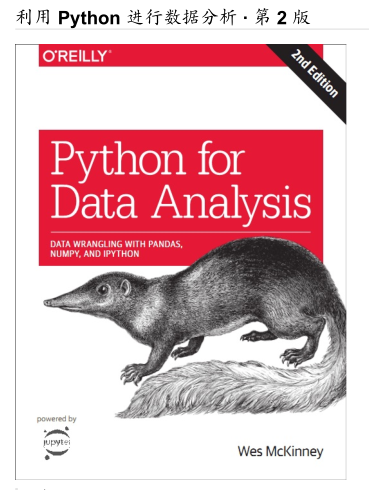
\includegraphics[width=.5\linewidth]{fig/book}
		\caption{书籍封面}
		\label{fig-book}
	\end{figure}
	\section{numpy基础}
	\subsection{创建ndarray}
	\begin{lstlisting}
		arr1.shape\\array
		asarray
		arange
		ones,ones_like
		zeros,zeros_like
		empty. empty_like.
		eye, identity
		数组转置和轴对称:
		arr.T
		arr.transpose
		arr.swapaxes
	\end{lstlisting}
	
%	\begin{figure}[htbp]
%		\centering
%		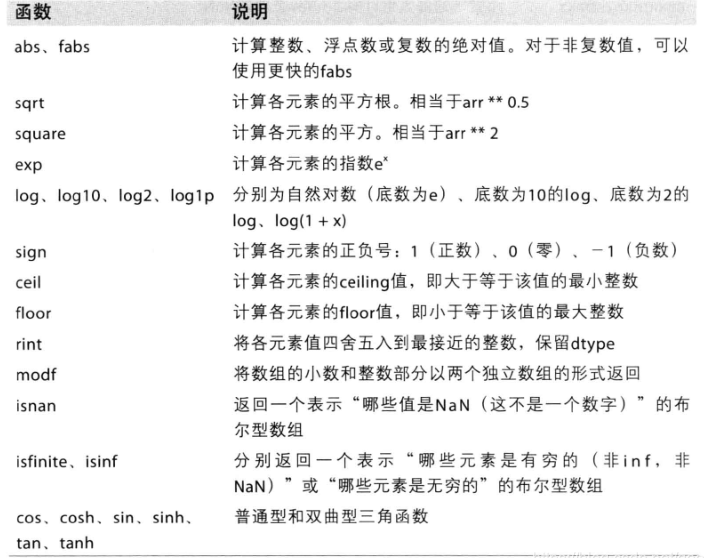
\includegraphics[height=6.0cm,width=9.5cm]{fig/np_ufunc}%fig2文件夹下的xbee.esp图片,
%		\caption{numpy中各种基础函数}
%	\end{figure}
%	
% 并排插入多张图,是再浮动提环境中,加入迷你页环境,然后再迷你页环境中进行图的掺入。
%	\begin{figure}[htbp]		
%		\begin{minipage}[t]{0.2\linewidth}			
%			\centering			
%			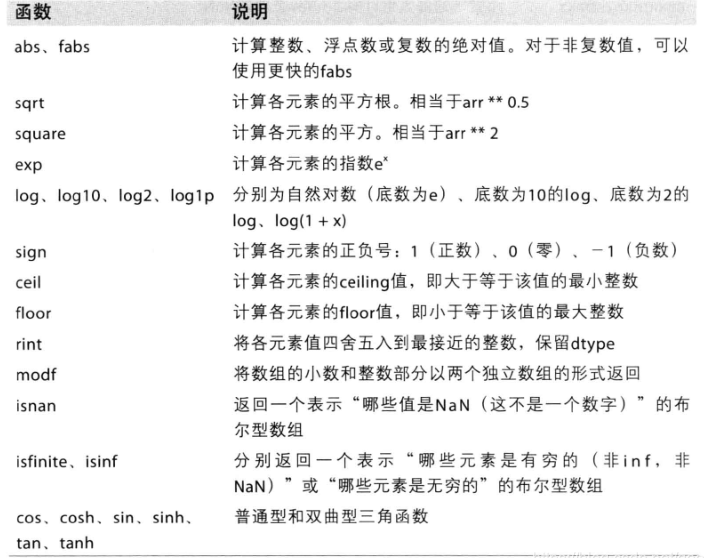
\includegraphics{fig/np_ufunc}			
%			\caption{Fatigue detection overview}			
%		\end{minipage}		
%		\hfill	
%		\begin{minipage}[t]{0.2\linewidth}		
%			\centering		
%			%\includegraphics[height=7.5cm,width=2.5cm]{fig2/tupianchuli1.eps}	
%			\caption{The image processing}			
%		\end{minipage}		
%		\hfill		
%		\begin{minipage}[t]{0.2\linewidth}		
%			\centering		
%			%\includegraphics[height=7.5cm,width=2.5cm]{fig2/tupianchuli1.eps}		
%			\caption{The image processing}		
%		\end{minipage}	
%	\end{figure}	
	
%	\begin{figure}
%		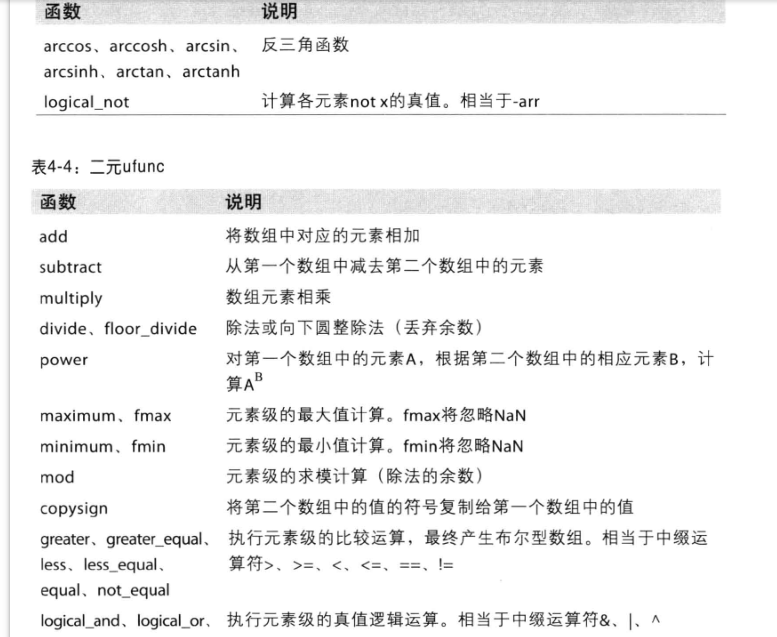
\includegraphics[height=6.0cm,width=9.5cm]{fig/np_2}
%		\caption{}
%	\end{figure}
\begin{figure}	
	\centering	
	\subfigure[1]{		
		\label{figa} %% label for first subfigure	
		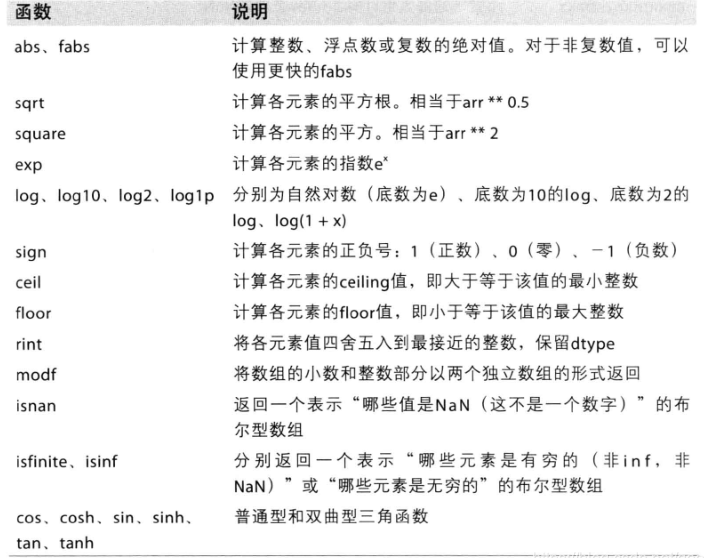
\includegraphics[width=1.5in]{fig/np_ufunc}}	
	\hspace{1in}	
	\subfigure[2]{	
		\label{fig:subfig:b} %% label for secondsubfigure	
		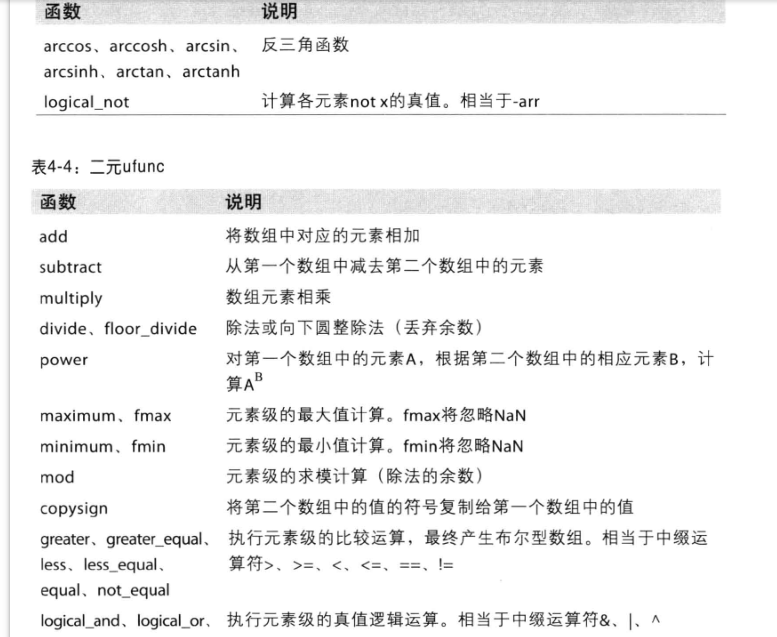
\includegraphics[width=1.5in]{fig/np_2}}	
	\caption{基础函数}
	\label{figb} %% label for entire figure	
\end{figure}	
	
	\subsection{利用数组进行数据处理}
	np.meshgrid 接收两个一维数组,产生两个二维矩阵。
	对应于所有的(x,y)对,产生的两个矩阵一个对第一个数组进行行重复,一个以列进行重复。两个矩阵凉凉对应后,就是所谓的网格点坐标对军阵。
	\begin{lstlisting}
		points = np.arange(-5,5,0.01)
		xs,ys = np.meshgrid(points, points)
		ys
		
		输出:
		ys:
		array([[-5.  , -5.  , -5.  , ..., -5.  , -5.  , -5.  ],
		[-4.99, -4.99, -4.99, ..., -4.99, -4.99, -4.99],
		[-4.98, -4.98, -4.98, ..., -4.98, -4.98, -4.98],
		...,
		[ 4.97,  4.97,  4.97, ...,  4.97,  4.97,  4.97],
		[ 4.98,  4.98,  4.98, ...,  4.98,  4.98,  4.98],
		[ 4.99,  4.99,  4.99, ...,  4.99,  4.99,  4.99]])
		xs:
		array([[-5.  , -4.99, -4.98, ...,  4.97,  4.98,  4.99],
		[-5.  , -4.99, -4.98, ...,  4.97,  4.98,  4.99],
		[-5.  , -4.99, -4.98, ...,  4.97,  4.98,  4.99],
		...,
		[-5.  , -4.99, -4.98, ...,  4.97,  4.98,  4.99],
		[-5.  , -4.99, -4.98, ...,  4.97,  4.98,  4.99],
		[-5.  , -4.99, -4.98, ...,  4.97,  4.98,  4.99]])
		z = np.sqrt(xs**2 + ys**2)
		输出:
		array([[7.07106781, 7.06400028, 7.05693985, ..., 7.04988652, 7.05693985,
		7.06400028],
		[7.06400028, 7.05692568, 7.04985815, ..., 7.04279774, 7.04985815,
		7.05692568],
		[7.05693985, 7.04985815, 7.04278354, ..., 7.03571603, 7.04278354,
		7.04985815],
		...,
		[7.04988652, 7.04279774, 7.03571603, ..., 7.0286414 , 7.03571603,
		7.04279774],
		[7.05693985, 7.04985815, 7.04278354, ..., 7.03571603, 7.04278354,
		7.04985815],
		[7.06400028, 7.05692568, 7.04985815, ..., 7.04279774, 7.04985815,
		7.05692568]])
		
		画图:
		plt.imshow(z,cmap=plt.cm.gray); plt.colorbar()
		plt.title('Image plot of $\sqrt{x^2+y^2}$ for a grid of values')
		
	\end{lstlisting}
	\begin{figure}[htbp]
		\centering
		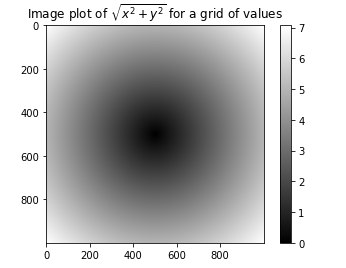
\includegraphics[]{fig/np_3}
		\caption{meshgird灰度图}
		\label{ifg-meshgrid}
	\end{figure}

\subsection{将条件逻辑表述为数组运算}
\emph{numpy.where(condition,x,y)} 函数是三元表达式 x if condition else y 的矢量化版本。

\begin{lstlisting}
	xarr = np.array([1.1, 1.2, 1.3, 1.4, 1.5])
	yarr = np.array([2.1, 2.2, 2.3, 2.4, 2.5])
	cond = np.array([True, False, True, True, False])
	#我们想要根据cond的值选取xarr和yarr,当cond的true,选取xarr的值,否则选取yarr的值。 
	result = [(x if c else y) for x, y, c in zip(xarr, yarr, cond)]
	结果:
	[1.1, 2.2, 1.3, 1.4, 2.5]
\end{lstlisting}
当我们使用多维数组的时候,上述处理方法不是很快,要快速处理的话,我们使用如下方法:
\begin{lstlisting}
	d = zip(xarr, yarr, cond)
	result = np.where(cond, xarr, yarr)
	result:
	array([1.1, 2.2, 1.3, 1.4, 2.5])
	
	from numpy.random import randn
	arr = randn(4,4)
	arr:
	array([[-1.00815132,  0.02094386, -1.40737364,  0.57612992],
	[-0.27886028,  0.76804402, -0.28459415, -1.75665045],
	[-0.39905925, -2.3398309 ,  0.26511772, -0.37557294],
	[ 0.44804335,  3.08441085,  0.7388182 , -0.5724736 ]])
	np.where(arr > 0, 2, -2) # 条件后边还可以直接跟标量。如果为矢量的话,那么维度就需要跟arr有相一致。
	array([[-2,  2, -2,  2],
	[-2,  2, -2, -2],
	[-2, -2,  2, -2],
	[ 2,  2,  2, -2]])
\end{lstlisting}

\subsection{数学和统计方法}
\emph{聚合运算:aggregation,约简 reduction
sum,mean,max,min,std,np.cumsum,np.cumprod....}
\emph{cumsum,cumprod} 都是不产生聚合效果的。

\begin{figure}[htbp]
	\centering
	\label{fig-juhehanshu}
	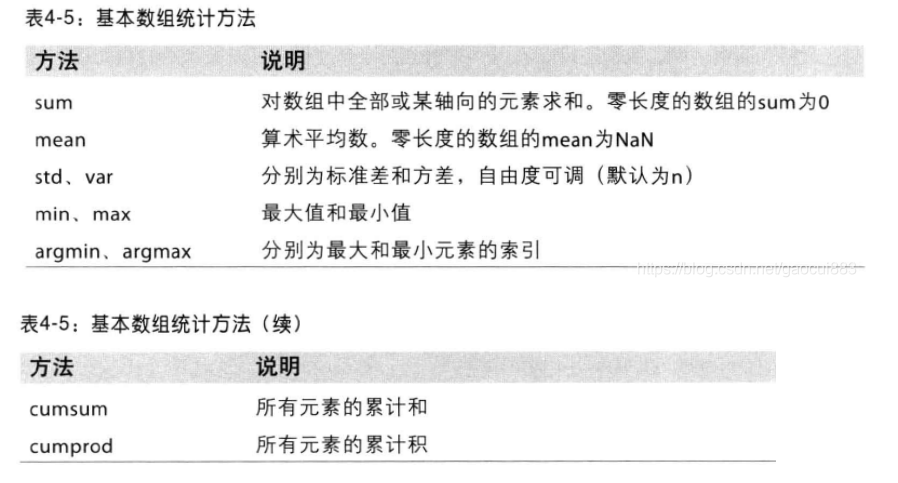
\includegraphics[width=4in]{fig/np_4}
	\caption{各种聚合和约简单函数}
\end{figure}
	
	\subsection{用于布尔型数组的方法}
	\begin{lstlisting}
		arr = randn(100)
		(arr > 0)
		输出:
		array([ True, False,  True, False,  True, False,  True, False, False,
		False,  True,  True, False,  True,  True,  True,  True, False,
		False,  True, False, False, False,  True,  True,  True,  True,
		False,  True, False, False, False,  True, False,  True,  True,
		False,  True, False, False, False,  True,  True, False,  True,
		False,  True, False, False, False,  True,  True,  True, False,
		False, False, False, False, False, False,  True, False, False,
		False, False, False,  True,  True,  True, False,  True, False,
		False,  True,  True, False,  True,  True,  True, False, False,
		False,  True, False,  True, False, False,  True,  True, False,
		False, False, False,  True,  True,  True, False,  True, False,
		True])
		统计ture的个数:
		(arr > 0).sum()
		默认将True当作1,将false当作0 来进行统计:
		46
	\end{lstlisting}
	
	np.any(),np.all,array.all(),array.any() 都是即可以根据轴axis来进行统计,也可以进行总体统计。
	\subsection{排序}
	\emph{arr.sort(axis=???)} 根据轴进行排序。\\
	\emph{np.unique()} 类似于python的\emph{set()}函数。\\
	\emph{np.in1d(ar1,ar2)} 测试集合1的成员是否再集合2中。
	\begin{lstlisting}
		values = np.array([6,0,3,2,5,6])		
		np.in1d(values, [2,3,5]) # 测试values的成员是否在当前集合中。
		输出:
		array([False, False,  True,  True,  True, False])
	\end{lstlisting} 
	\begin{figure}[htbp]
		\centering
		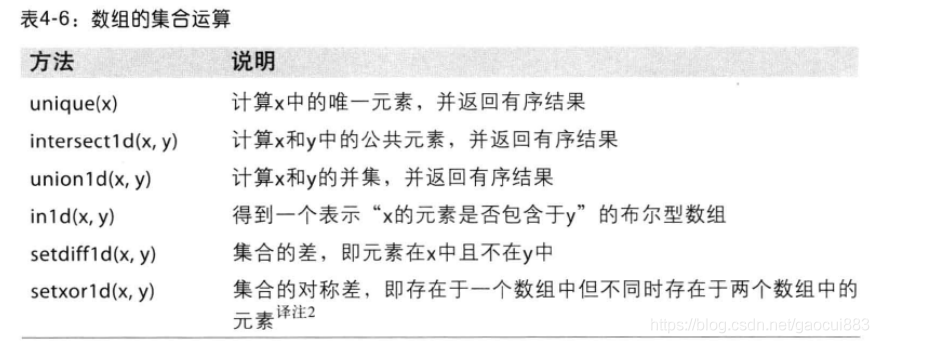
\includegraphics[width=4in]{fig/np_5}
		\caption{数组集合运算}
		\label{fig-jiheyunsuan}
	\end{figure}
	\subsection{用于数组的文件输入输出}
	\begin{lstlisting}
		arr = np.arange(10)
		数组的保存于读取:
		np.save('some_array',arr)
		np.load('some_array.npy')
		多个数组保存于读取:
		np.savez('some_array.npz',a=arr,b=arr) # 将两个数组压缩到一起存储。
		arch = np.load('some_array.npz')
		arch['a']
	\end{lstlisting}
	
	\subsection{存取文本文件}
	\noindent\verb|read_csv, rea_table|\\
	\verb|arr = np.loadtxt('array_ex.txt',delimiter=',')|\\
	当然这些都是针对纯数组文件的。
	
	\subsection{线性代数}
	\begin{lstlisting}
		x = np.array([[1.,2.,3.],[4.,5.,6.]])
		y = np.array([[6.,23.],[-1,7],[8,9]])
		输出:
		[[1. 2. 3.]
		[4. 5. 6.]]
		[[ 6. 23.]
		[-1.  7.]
		[ 8.  9.]]
		x.dot(y),np.dot(x,y)
		分解,行列式,求逆运算,方程组的解。
		from numpy.linalg import inv,qr
		mat = x.T.dot(x)
		inv(mat)
		mat.dot(inv(mat))
		计算矩阵的qr分解:
		q,r = qr(mat)
		因为q是正交的,所以q.dot(q.T) 为单位矩阵。
		因为r为对角的,所以 inv(r).dot(r)也是单位。从而应用q,r,就可以计算多元方程组。
		ax = b
		
		a= qr
		
		x = inv(r).dot(q.T).dot(b)
	\end{lstlisting}
	\begin{figure}[htbp]
		\centering
		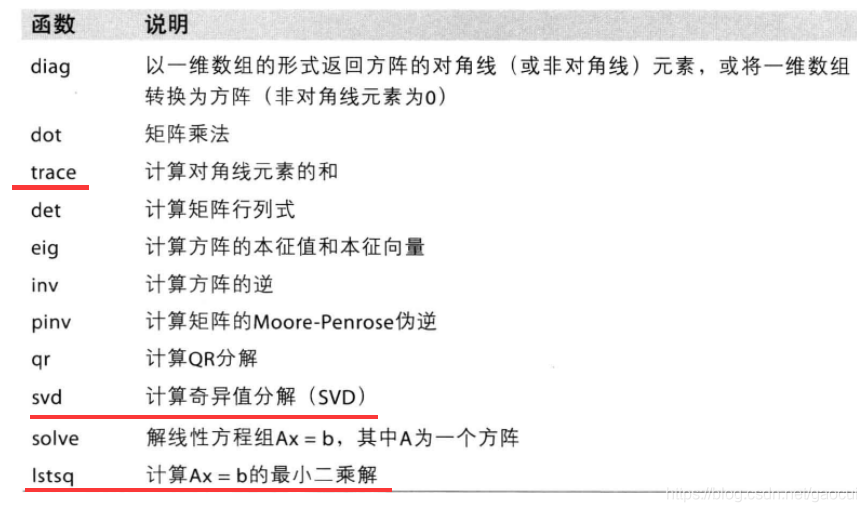
\includegraphics[width=\linewidth]{fig/np_6}
		\caption{常用线性函数}
	\end{figure}
	\subsection{随机数生成}
	\noindent 随机高斯分布生成:
	\begin{lstlisting}
		samples = np.random.normal(size=(4,4))
	\end{lstlisting}

%	\begin{figure}
%		\subfigure[1]{
%			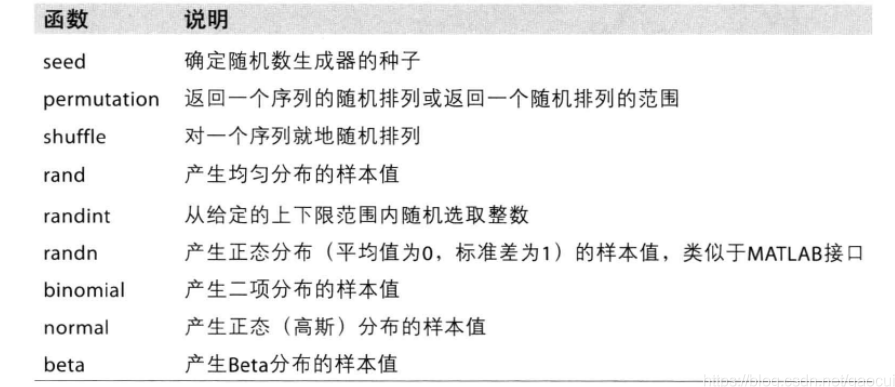
\includegraphics[width=1.6in]{fig/np_7}}
%		\vspace{1em}
%		\subfigure[2]{
\includegraphics[width=1.6in]{fig/np_8}}
%		\caption{np.random.xx 函数}
%	\end{figure}
	\begin{figure}[htbp]
		\centering
	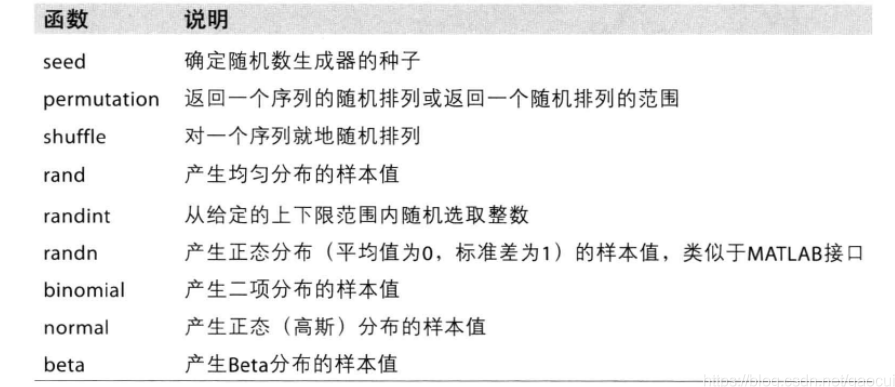
\includegraphics[width=\linewidth]{fig/np_7}
	\caption{常用的random函数1}
	\end{figure}
	\begin{figure}[htbp]
	\centering
	
\includegraphics[width=\linewidth]{fig/np_8}
	\caption{常用的random函数2}
\end{figure}

\subsection{范例,随机漫步}
\begin{lstlisting}
	import random
	position = 0
	walk = [position]
	steps = 1000
	for i in range(steps):
	step = 1 if random.randint(0,1) else -1
	position += step
	walk.append(position)
\end{lstlisting}
	\begin{figure}[htpb]
		\centering
		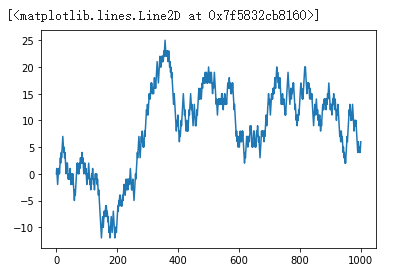
\includegraphics[width=3in]{fig/np_9}
		\caption{随机漫步效果}
	\end{figure}
用np的方法来实现:
\begin{lstlisting}
	nsteps = 1000
	产生两个数0 1 :
	draws = np.random.randint(0,2,size=nsteps)
	判断方向:
	steps = np.where(draws >0,1,-1)
	进行走动:
	walk = steps.cumsum()
	判断最远和最近:
	walk.min()
	walk.max()
	画出图像:
	plt.plot([x for x in range(nsteps)],walk)
	第一次离0点距离大于10:
	a = np.abs(walk) >= 10
	找出第一次的坐标:
	a.argmax()
\end{lstlisting}	

\subsection{一次模拟多个随机漫步}
\begin{lstlisting}
	nwalks = 5000
	nsteps = 1000
	draws = np.random.randint(0,2,size=(nwalks, nsteps))
	steps = np.where(draws > 0, 1, -1)
	walks = steps.cumsum(1) #在列方向进行累加。
	walks.max()
	walks.min()
	hist30 = (np.abs(walks)>= 30).any(1)
	多少次随机漫步穿过了30
	hist30.sum()
	找出那些穿过30的随机漫步,第一次穿过30的索引。
	crossing_times = (np.abs(walks[hist30]) >=30).argmax(1)
	对他们求平均值。
\end{lstlisting}

\section{pandas 入门}
\subsection{Series Class}
\begin{lstlisting}
	from pandas import Series, DataFrame
	import pandas as pd
	obj = Series([4,7,-5,3])
	obj.values
	obj.index
	obj2 = Series([4,7,5,3], index=['a', 'b', 'c', 'd'])
	结果:
	a    4
	b    7
	c    5
	d    3
	dtype: int64
	
	obj2['d']  3
	字典和series转换:
	sdata = {'ohi':3500, 'texa':7100, 'orgen':1900, 'utah':4000}
	obj3 = Series(sdata)
	:
	ohi      3500
	texa     7100
	orgen    1900
	utah     4000
	dtype: int64
	列表当作index:
	states = ['aiaang','ohi',  'orgen', 'utah']
	obj4 = Series(sdata, index=states)
	判断series各个值是否为null:
	pd.isnull(obj4)
	pd.notnull()
	series相加:pandas会根据索引自动进行配对,没有配对成功的结果做nan
	
	series的name属性:
	obj4.name = 'population'
	obj4.index.name = 'state'
	::
	state
	aiaang       NaN
	ohi       3500.0
	orgen     1900.0
	utah      4000.0
	Name: population, dtype: float64
\end{lstlisting}

\subsection{DataFrame Class}
\begin{lstlisting}
	import numpy as np
	import pandas as pd
	from pandas import Series
	from pandas import DataFrame
	# 传入由等长列表组成的字典,来构建DataFrame
	data = {'state': ['Ohio','Ohio','Ohio','Nevada','Nevada'],
	'year': [2000, 2001, 2002, 2001, 2002],
	'pop': [1.5, 1.7, 3.6, 2.4, 2.9]}
	frame = DataFrame(data)
	state	year	pop
	0	Ohio	2000	1.5
	1	Ohio	2001	1.7
	2	Ohio	2002	3.6
	3	Nevada	2001	2.4
	4	Nevada	2002	2.9
\end{lstlisting}
可以向上边一样,之际由字典来构成一个dataframe:字典key自动当成columns。
索引自动生成。
也可以自动改变索引:
\lstinline|DataFrame(data, columns=['year', 'state', 'pop'])|	\\
自己设定index,columns名字:\\
\lstinline|frame2 = DataFrame(data, columns=['year', 'state', 'pop', 'debt'], index=['one', 'two', 'three', 'four', 'five'])|

\begin{lstlisting}
df:列名列表:
	frame2.columns
Index(['year', 'state', 'pop', 'debt'], dtype='object')

dataframe可以转置:
frame3 = DataFrame(pop)
frame3
Nevada	Ohio
2001	2.4	1.7
2002	2.9	3.6
2000	NaN	1.5
frame3.T
2001	2002	2000
Nevada	2.4	2.9	NaN
Ohio	1.7	3.6	1.5

frame3.index.name = 'year'
frame3.columns.name = 'state'
\end{lstlisting}
\begin{figure}[htpb]
	\centering
	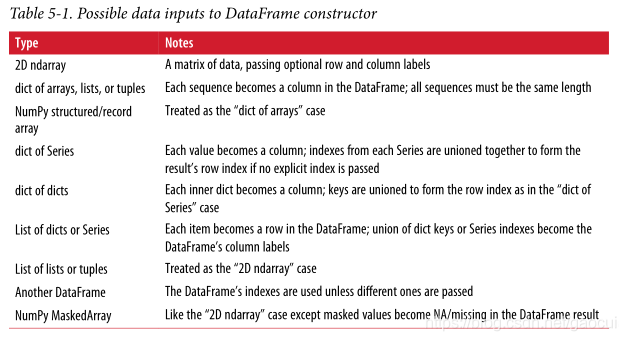
\includegraphics[width=\linewidth]{fig/df1}
	\caption{所有可以传给dataframe的值}
\end{figure}

\subsection{Index Objects 索引对象}
比如:\lstinline|frame3.columns| 就是index object索引对象。\\
然后可以判断这个索引对象内是否含有某个对象:'Ohio' in frame3.columns : true

\begin{figure}[hpb]
	\centering
	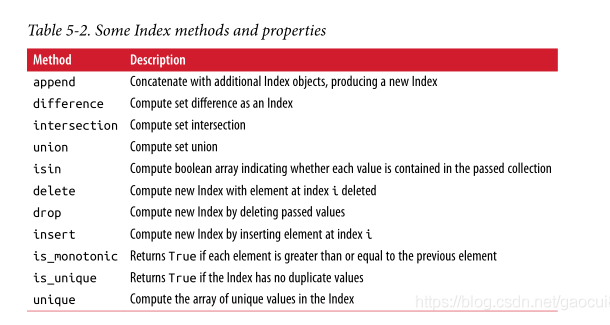
\includegraphics[width=\linewidth]{fig/df2}
	\caption{index对象的各种方法和属性}
\end{figure}

\subsection{Essential Functionality}
\subsection{reindexing 索引重建}
\begin{lstlisting}
	obj = pd.Series([4.5, 7.2, -5.3, 3.6],index=['d', 'b', 'a', 'c'])
	obj2 = obj.reindex(['a','b','c','d','e'])
	obj3 = pd.Series(['blue', 'purple', 'yellow'],index=[0,2,4])
	obj3.reindex(range(6), method='ffill') #range boject	
\end{lstlisting}

\subsection{Dropping Entries from an Axis}
\noindent Dropping Entries from an Axis\\
根据轴来删除条目\\
obj.drop(labels=None, axis=0, index=None, columns=None, level=None,\\ inplace=False, errors='raise')\\
\begin{lstlisting}
	obj= pd.Series(np.arange(5.0),index=['a','b','c','d','e'])
	new_obj = obj.drop('a')
	data = pd.DataFrame(np.arange(16).reshape(4,4), index=['Ohio', 'Colorada', 'Utah', 'New York'],
	columns=['one', 'two', 'three', 'four'])
	data.drop(['Colorada', 'Ohio'])
	data.drop(['one','two'], axis= 1)
	data.drop(columns=['one', 'two'])
	data.drop(index=['Ohio'], columns=['two'], inplace=True)
\end{lstlisting}

\subsection{Indexing, Selection, and Filtering索引、选择和筛选}
\subsubsection{indexing}

\begin{lstlisting}
Series:
	obj = pd.Series(np.arange(4.), index=['a', 'b', 'c', 'd'])
	obj[['a','c']]
	obj[[1,3]]
	obj[obj < 2]
	obj['a':'c']
	obj['a':'c'] = 100
DataFrame:
	data = pd.DataFrame(np.arange(16).reshape(4,4), index=['Ohio', 'Colorada', 'Utah', 'NewYork'],
	columns= ['one', 'two', 'trhee', 'four'])
	data
	data.loc['Ohio']
	data['two']
	data[['trhee','two']]
	data[:2]
	data[:1]
	data[data['trhee'] > 5 ]
	data < 5
	data[data < 5] = 0 # like numpy case.
		
\end{lstlisting}

\subsubsection{Selection with loc and iloc (loc,iloc)}
loc用索引名字符,iloc用索引位置:
\begin{lstlisting}
	Selection with loc and iloc (loc,iloc)
	data.iloc[2,[3,0,1]]
	data.iloc[2]
	data.loc[:'Utah', 'two']
	data.loc['Utah', 'two']
	data.iloc[:,:3]
	one	two	trhee
	Ohio	0	0	0
	Colorada	0	5	6
	Utah	8	9	10
	NewYork	12	13	14
	
\end{lstlisting}
\begin{figure}
	\centering
	\subfigure{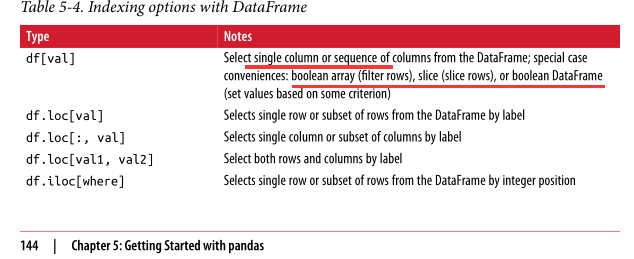
\includegraphics[width=\linewidth]{fig/df3}}
	\subfigure{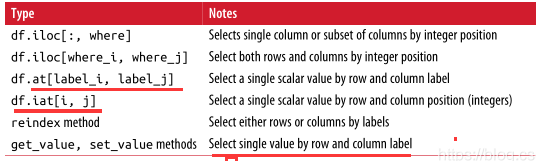
\includegraphics[width=\linewidth]{fig/df4}}
	\caption{DataFrame索引}
\end{figure}

\subsubsection{Integer Indexes 整数索引}
\begin{lstlisting}
	ser = pd.Series(np.arange(6.0))
	ser.loc[:1]
	ser2.iloc[:2]
\end{lstlisting}

\subsection{Arithmetic and Data Alignment. 算法和数据对齐}
意思就是,在进行运算的时候,dataframe和Series 可以自动进行对齐,对不齐的部分结果为0.


\subsection{Arithmetic methods with fill values 填充值的算数方法}
一般来说直接用“+-*/” 方法,但是没法对不对齐的部分进行填充。\\
但是如果用相应的函数运算的话,那么可以进行一些非对齐NAN填充。\\
\begin{figure}[hbtp]
	\centering
	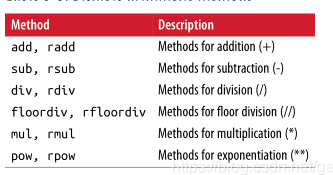
\includegraphics[width=\linewidth]{fig/df5}
	\caption{相应的计算函数}
\end{figure}
用着写函数来对dataframe进行运算的时候,可以传一个对应的\verb|fill_value|参数。

\subsection{Operations between DataFrame and Series}
默认serie和dataframe加减,自动进行行广播。
	
\begin{lstlisting}
	frame = df(np.arange(12.0).reshape((4,3)),
	columns= list('bde'),
	index=['Utah', 'Ohio', 'Texas', 'Oregon'])
	series = frame.iloc[0]
	
	frame - series 进行行广播,当然无法自动对齐,也就是没有对应列的进行NAN赋值。
	b     d     e
	Utah    0.0   1.0   2.0
	Ohio    3.0   4.0   5.0
	Texas   6.0   7.0   8.0
	Oregon  9.0  10.0  11.0
	
	series2 = pd.Series(range(3), index= list('bef'))
	
	frame + series2
	b	d	e	f
	Utah	0.0	NaN	3.0	NaN
	Ohio	3.0	NaN	6.0	NaN
	Texas	6.0	NaN	9.0	NaN
	Oregon	9.0	NaN	12.0	NaN	
\end{lstlisting}


\subsection{Function Application and Mapping 函数应用与映射}
\begin{lstlisting}
	frame = df(np.random.randn(4,3), columns=list('bde'), index=['Utah', 'Ohio', 'Texas', 'Oregon'])
	
	np.abs(frame)
	
	默认取列:因为一般将列当作特征,行当作样本行:
	f = lambda x: x.max() - x.min()
	frame.apply(f)
	
	frame.apply(f, axis = 'columns')
	frame.apply(f, axis= 1)
传递的参数不是表格的单个元素,而是整个表格的列或者行,或者整个表格:
	def f(x):
		return pd.Series([x.min(), x.max()], index=['min', 'max'])
	frame.apply(f)
表格的形状不改变,只是改变了表格元素对应值:用map和applymap:
	format = lambda x: '%2f' % x
	frame.applymap(format)
	
	frame['e'].map(format)
	
	
\end{lstlisting}

\subsection{Sorting and Ranking}

\begin{lstlisting}
	Signature: frame.sort_index(axis=0, level=None, ascending=True, inplace=False, kind='quicksort', na_position='last', sort_remaining=True, ignore_index: bool=False)
	
	Docstring: Sort object by labels (along an axis).
	
	Signature: obj.sort_values(axis=0, ascending=True, inplace=False, kind='quicksort', na_position='last', ignore_index=False)
	
	Docstring: Sort by the values.
	
	还有一种:obj.rank(method='first')
	排出的是对应数据的位次。
\end{lstlisting}

\subsection{Axis Indexes with Duplicate Labels 具有重复标签的轴索隐}
obj = sr(range(5), index=list('aabbc'))



\subsection{Summarizing and Computing Descriptive Statistics 汇总计算描述性统计}

意思就是像:sum,mean,maxa,min之类的都是汇总计算描述性统计。\\

\begin{lstlisting}
	df1.mean(axis= 1,skipna= False) #不能忽略NA\\
	df1.idxmax()\\
	df1.cumsum() 
	df1.describe()
\end{lstlisting}

\begin{figure}[hbtp]
	\centering
	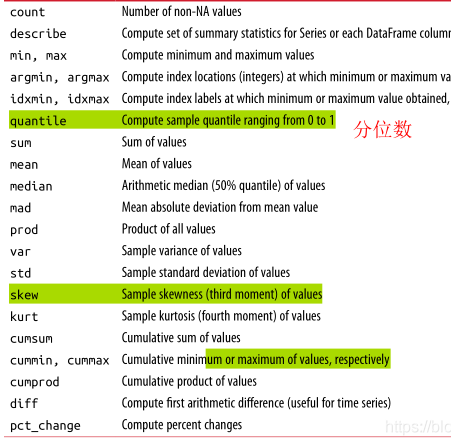
\includegraphics[width=\linewidth]{fig/df6}
	\caption{各种统计函数}
	\label{fig-tongjihanshu}
\end{figure}

\subsection{Correlation and Covariance 相关以及协方差}
\begin{lstlisting}
	import pandas_datareader.data as web
	从雅虎网站读取股票收盘价格信息:
	all_data = {ticker:web.get_data_yahoo(ticker) for ticker in ['AAPL', 'IBM', 'MSFT', 'GOOG']}
	price = DF({ticker: data['Adj Close'] for ticker, data in all_data.items()}) #收盘价
	volume = DF({ticker: data['Volume'] for ticker,data in all_data.items()}) #成交量。
	
	变换量百分比:
	returns = price.pct_change()
	
	AAPL	IBM	MSFT	GOOG
	Date				
	2020-08-03	0.025198	0.011144	0.056241	-0.005739
	2020-08-04	0.006678	0.012308	-0.015009	-0.006430
	2020-08-05	0.003625	-0.003099	-0.001641	0.005898
	2020-08-06	0.034889	0.005341	0.016014	0.017976
	2020-08-07	-0.022736	0.003775	-0.017888	-0.003740
	计算不同股票涨跌协方差,相关性:
	returns['IBM'].corr(returns['GOOG'])
	
	returns['IBM'].cov(returns['GOOG'])
	产生协方差和相关矩阵:
	returns.cov()
	returns.corr() 
	returns.corrwith(returns.IBM)
	计算价格涨跌和成交量的关系:
	returns.corrwith(volume)
\end{lstlisting}

\subsection{Unique Values, Value Counts, and Membership}
\begin{figure}[htbp]
	\centering
	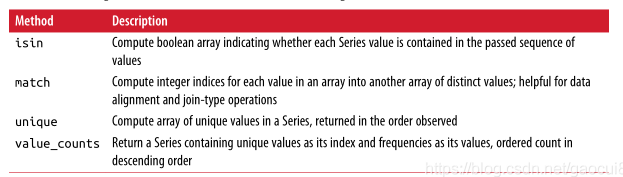
\includegraphics[width=\linewidth]{fig/df7}
	\caption{unique,valuecount,membership}
	\label{fig-unique_function}
\end{figure}

\section{Data Loading, Storage, and File Formats}
pandas features a number of functions for reading tabular data as a DataFrame object. Table \verb|6-1| summarizes some of them, though \verb|read_csv| and  \verb|read_table| are likely the ones you’ll use the most.
\begin{figure}[hbpt]
	\centering
	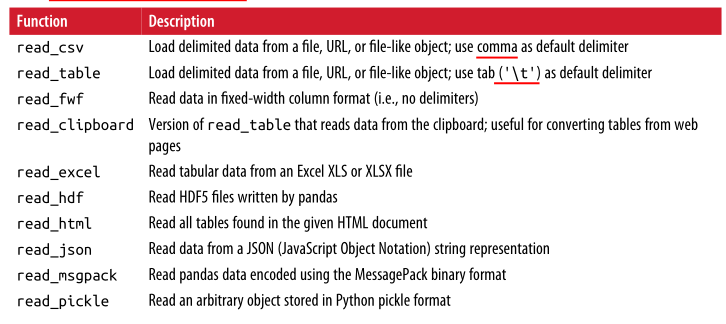
\includegraphics[width=\linewidth]{fig/df8}
	\caption{parsingfunction in pandas}
		\label{fig-csv,table}
\end{figure}
\subsection{Reading and Writing Data in Text Format}
\noindent indexing: can treat one or more columns as the returened DataFrame\\
type inference an data conversion:\\
detectime parsing\\
iterating\\
unclean data issues\\

\begin{lstlisting}
df = pd.read_csv('/content/sample_data/ex1.csv')
pd.read_table('/content/sample_data/ex1.csv', delimiter=',')
pd.read_csv('/content/sample_data/ex2.csv', header=None)
pd.read_csv('/content/sample_data/ex2.csv', names=list('abcde'))
names = ['a','b','c','d','message']
pd.read_csv('/content/sample_data/ex2.csv',names=names, index_col='message')# 用names中的message列做为index。

parsed = pd.read_csv('/content/sample_data/csv_mindex.csv', index_col=['key1','key2']) #用两列做二级索引。

list(open('/content/sample_data/ex3.txt'))
result = pd.read_table('/content/sample_data/ex3.txt',sep='\s+')

pd.read_csv('/content/sample_data/ex4.csv', skiprows=[0,2,3])

result = pd.read_csv('/content/sample_data/ex5.csv', na_values=['NULL'])
result = pd.read_csv('/content/sample_data/ex5.csv', na_values={'message':['foo', 'NA'], 'something':['two']})
pd.read_csv('ex6.csv', nrows=5)

chunker = pd.read_csv('ex6.csv', chunksize=1000) # chunker is iter
tot = Series([])
for piece in chunker:
	tot =tot.add(piece['key'].value_counts(), fill_value=0)  #每个块1000个,每次统计1000个,将最后的结果相加,就是总体的。

tot = tot.sort_values(ascending=False)
\end{lstlisting}
\begin{figure}
	\centering
	\subfigure[1]{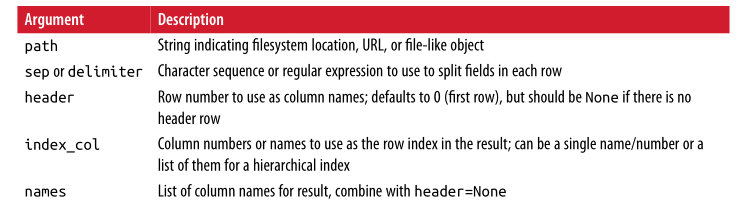
\includegraphics[width=\linewidth]{fig/df9}}
	\subfigure[2]{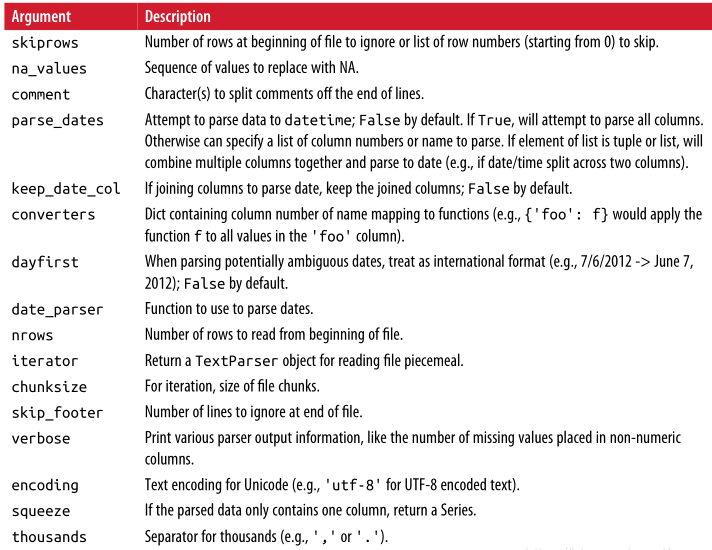
\includegraphics[width=\linewidth]{fig/df10}}
	\caption{read\_csv的参数}
	\label{fig-csvparams}
\end{figure}

\subsection{Writing Data to Text Format}
\begin{lstlisting}
	import sys
	data.to_csv(sys.stdout, sep="|")
	data.to_csv(sys.stdout, sep='|', na_rep='NULL')
	存储后没有索引:
	data.to_csv(sys.stdout, index=False,header=False, sep='|', na_rep='null')
	有设置列号:
	data.to_csv(sys.stdout, index=False, columns=['a','b'])
	设置时间索引:
	dates = pd.date_range('1/1/2000', periods=7)
	ts = pd.Series(np.arange(7), index=dates)
	ts.to_csv(sys.stdout)	
	
\end{lstlisting}


\subsection{Working with Delimited Formats重点}

\begin{lstlisting}
import csv后读取:
	f = open('ex7.csv')
	reader = csv.reader(f)
	for line in reader:
		print(line)
reader方法:	
	with open('ex7.csv') as f:
		lines = list(csv.reader(f))
	
	header,values = lines[0], lines[1:]
	data_dict = {h:v for h,v in zip(header,zip(*values))} ######################
	data_dict
自定以分隔spliter:	
#simple subclass csv.Dialect
class my_dialect(csv.Dialect):
	lineterminator = '\n'
	delimiter = ';'
	quotechar = '"'
	quoting = csv.QUOTE_MINIMAL
f = open('ex7.csv')
reader = csv.reader(f, dialect=my_dialect)	
	
\end{lstlisting}
\subsection{JSON Data}
\begin{lstlisting}
读取:
	import json
	result = json.loads(obj)
	result
装载(载入):
	asjson = json.dumps(result)
因为json 是字典形式的,所以天生就可以转换成dataframe

用字典的key来做columns:
siblings = DF(result['siblings'], columns= ['age','name','pets'])
	age	name	pets
0	30	Scott	[Zeus, Zuko]
1	38	Katie	[Sixes, Stache, Cisco]
\end{lstlisting}

\verb|pandas.read_json| 可以自动的将JSON 数据按特定顺序排列成dataframe\\
\verb|data = pd.read_json('example.json')|\\
\verb|data.to_json()| 也可以将dataframe转换成为json\\

\subsection{XML and HTML : Web Scraping}
\begin{lstlisting}
读取银行倒闭信息:
	tables = pd.read_html('fdic_failed_bank_list.html')
	时间信息转换标准时间格式:
	cl = pd.to_datetime(x['Closing Date'])
	从是按列,抽取年份:
	cl.dt.year
	统计倒闭数量:
	cl.dt.year.value_counts()	
\end{lstlisting}

\subsection{Parsing XML with lxml.objectify}
\noindent 分层,嵌套的文件形式。\\
\begin{lstlisting}
	from lxml import objectify
	path = 'Performance_MNR.xml'
	parsed = objectify.parse(open(path))    #############important way.
	root = parsed.getroot()
	
	data = []
	skip_fields = ['PARENT_SEQ', 'INDICATOR_SEQ','DESIRED_CHANGE', 'DECIMAL_PLACES']
	
	for elt in root.INDICATOR:
		el_data = {}
		for child in elt.getchildren():
			if child.tag in skip_fields:
				continue
			el_data[child.tag] = child.pyval #child.tag标签和pyval 值,存储。作为一个字典。
		data.append(el_data)
\end{lstlisting}

\subsection{Binary Data Formats}
pandas 有两个函数:\verb|to_pickle and read_pickle| 可以将数据简单的存储为二进制文件。
\begin{lstlisting}
	frame = pd.read_csv('ex1.csv')
	print(frame)
	frame.to_pickle('ex1_frame_pickle')
	pd.read_pickle('ex1_frame_pickle')
	
	a	b	c	d	message
	0	1	2	3	4	hello
	1	5	6	7	8	world
	2	9	10	11	12	foo
\end{lstlisting}
 
\subsection{Using HDF5 Format}

\begin{lstlisting}
	frame = pd.DataFrame({'a':np.random.randn(100)})
	store = pd.HDFStore('mydata.h5')
	store['obj1'] = frame
	obj2为。
	store.put('obj2',frame,format='table')
	frame.to_hdf('mydata.h5','obj3',format='table')
	简便的方法:
	pd.read_hdf('mydata.h5', 'obj3', where=['index > 10 and index < 20'],mode='r+')
	
	
\end{lstlisting}



\subsection{Reading Microsoft Excel Files}
\begin{lstlisting}
	xlsx = pd.ExcelFile('ex1.xlsx')
	pd.read_excel(xlsx,'Sheet1')
	
	简便的方法:
	frame = pd.read_excel('ex1.xlsx', 'Sheet1')
	写入:
	writer = pd.ExcelWriter('ex2.xlsx')
	frame.to_excel(writer, 'Sheet1')
	writer.save()
	简便的写法:
	frame.to_excel('ex2.xlsx','Sheet2')
\end{lstlisting}


\subsection{Interacting with Web APIs}
requests.get() 网址信息,得到.json()对象。所以可以直接于daframe转换。
\begin{lstlisting}
	import requests
	url = 'https://api.github.com/repos/pandas-dev/pandas/issues'
	resp = requests.get(url)
	issues = DF(data, columns=['number', 'title', 'labels', 'state','url'])
	issues.head()
\end{lstlisting}


\subsection{Interacting with Databases}
与数据库对象进行互动:
\begin{lstlisting}
	import sqlite3
	query = '''
	CREATE TABLE test
	(a VARCHAR(20), b varchar(20), c real, d integer);'''
	创建和连接数据库:
	con = sqlite3.connect('mydata.sqlite')
	执行创建表:
	con.execute(query)
	con.commit()
	
	data = [('Atlanta', 'Georgia', 1.25, 6),
	('Tallahassee', 'Florida', 2.6, 3),
	('Sacramento', 'California', 1.7, 5)]
	stmt = "INSERT INTO test VALUES(?, ?, ?, ?)"
	多次执行命令:
	将data插入到test表格:
	con.executemany(stmt, data)
	con.commit()
	
	读取数据库:
	cursor = con.execute('select * from test')
	rows = cursor.fetchall()
	
	魔术方法:
	import sqlalchemy as  sqla
	
	db = sqla.create_engine('sqlite:///mydata.sqlite')
	pd.read_sql('select * from test',db)
\end{lstlisting}

\section{数据清洗与准备}
\subsection[数据缺失处理]{Handling Missing Data}
\begin{lstlisting}
	string_data.isnull()
	丢弃缺失数据:
	data[data.notnull()]
	data.dropna(axis, how,thresh, subset,inplace)
	(可以按行丢弃或者列丢弃)
	
	Filling In Missing Data 填充
	
\end{lstlisting}
\begin{figure}[htpb]
	\centering
	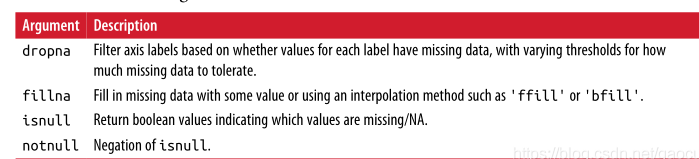
\includegraphics[width=\linewidth]{fig/na1}
	\caption{缺失数据函数}
	\label{fig-missingdata}
\end{figure}
\begin{figure}
	\centering
	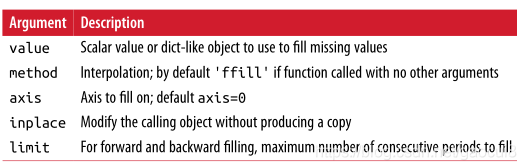
\includegraphics[width=\linewidth]{fig/na2}
	\caption{数据填充函数}
	\label{fig-fillna}
\end{figure}

\begin{lstlisting}
	df.fillna(value=none, method=none, axis=none,inplace, limite,downcast)
	value 可以指定填充的值,也可以指定相应的填充索引列或者行。
\end{lstlisting}

\subsection{Data Transformation}
\subsubsection{数据冗余}
\verb|duplicated(subset, keep:first,last)|  标记冗余数据的位置,只有一个会标记为true,其他为false表示冗余。
\begin{lstlisting}
	data.duplicated()
	data.drop_duplicates() 丢球冗余数据。
	data.drop_duplicates(['x','y'], keep='first'/'last') 丢弃x列的冗余数据,其他列冗余不冗余不管。
	
\end{lstlisting}
\subsubsection[基于索引的转换]{Transforming Data Using a Function or Mapping}

\begin{lstlisting}
data:
food	ounces
0	bacon	4.0
1	pulled pork	3.0
2	bacon	12.0
3	Pastrami	6.0
4	corned beef	7.5
5	Bacon	8.0
6	pastrami	3.0
7	honey ham	5.0
8	nova lox	6.0

	meat_to_animal = {
	'bacon':'pig',
	'pulled pork':'pig',
	'pastrami':'cow',
	'corned beef':'cow',
	'honey ham':'pig',
	'nova lox':'salmon'
	}
	lowercased = data['food'].str.lower()
	
data['animal'] = lowercased.map(meat_to_animal)
data['meat2'] = data['food'].map(lambda x: meat_to_animal[x.lower()])	
\end{lstlisting}



\subsubsection{Replicing Values}
数据值的替换。关键字: \verb|replace|

\begin{lstlisting}
	data.replace(-999, np.nan)
	data.replace([-999,-1000], ['xx','yy'])
	data.replace({-999:'xxxx', -1000:'yyyy'})
\end{lstlisting}

\subsubsection[改变索引名称]{Renaming Axis Indexes}
可以用map
\begin{lstlisting}
	tansform = lambda x:x[:4].upper()
	data.index.map(tansform)
	data.index = data.index.map(lambda x:x[:4].upper())
	data.columns = data.columns.map(lambda x:x[:].upper())
	k = data.rename(index = str.title, columns= str.lower)
	data.rename(index={'OHIO':'fuck'}, columns={'ONE':111})	
\end{lstlisting}
\subsubsection[离散与分组]{Discretization and Binning}	

\begin{lstlisting}
	cats = pd.cut(ages, bins)
	cats.codes
	cats.categories
	pd.value_counts(cats)
	
\end{lstlisting}
\subsubsection{检测和过滤异常}

\begin{lstlisting}
	col[np.abs(col) > 3]
	data[(np.abs(data) >3).any(axis = 1)]
	data[np.abs(data) >3] = np.sign(data)*3 	
\end{lstlisting}
\subsubsection{排列和随机抽样}
\begin{lstlisting}
	df = pd.DataFrame(np.arange(5*4).reshape((5,4)))
	从1-5随机抽取:
	sampler = np.random.permutation(5)
	按行随机抽取:
	df.take(sampler)
	df.iloc[sampler] 
	
	pandas里也有随机:
	df.sample(n=2) 随机抽两行。
	
	可以重复抽取:
	choices = Series([5, 7, -1, 6, 4])
	draws = choices.sample(n=10, replace= True)
\end{lstlisting}

\subsubsection{指示器和哑变量}

\begin{lstlisting}
	df = pd.DataFrame({'key': ['b', 'b', 'a', 'c', 'a', 'b'],
	'data1': range(6)})
	pd.get_dummies(df['key'],prefix='key')
a	b	c
0	0	1	0
1	0	1	0
2	1	0	0
3	0	0	1
4	1	0	0
5	0	1	0
		df_with_dummy = df[['data1']].join(dummies)


不用get_dummies的例子:		
mnames = ['movie_id', 'title', 'genres']
movies = pd.read_table('movies.dat', sep='::',header=None, names=mnames)
# 我们现在想做的工作是什么???
# 我们需要制作一个dataframe,用来显示这些不同的电影的风格,纵坐标是电影,横坐标风格,1表示该电影是此风格,否则为0

# 首先找出一共的风格数,并对其进行统计

all_genres = []
for x in movies.genres:
all_genres.extend(x.split('|')) #将各个风格进行分割,并且添加到all——genres中genres = pd.unique(all_genres)
from pandas import DataFrame as DF
zero_matrix = np.zeros((len(movies), len(genres)))
dummies = DF(zero_matrix, columns = genres)

# 下一步就是根据电影中的gernes 进行填写即可。

for i,gen in enumerate(movies.genres):
	indices = dummies.columns.get_indexer(gen.split('|')) #得到电影的风格索引。
	#根据这个索引进行填写为1.
	dummies.iloc[i, indices] = 1.0

movies_windic = movies.join((dummies.add_prefix('Genre_')))

		
\end{lstlisting}

\subsection{string 相关操作}
\begin{lstlisting}
	str.split()
	reslut2 = "::".join(pieces)
	val.index(',')
	val.find(',')
	val2 = val.replace(",", '::::')
	val.replace(",","") # 用来删除逗号。
	val.rjust(14, '&')
	val.ljust(15, "*")
	data.str.contains('gmail')
	
	
	
	
\end{lstlisting}
\begin{figure}[htpb]
	\centering
	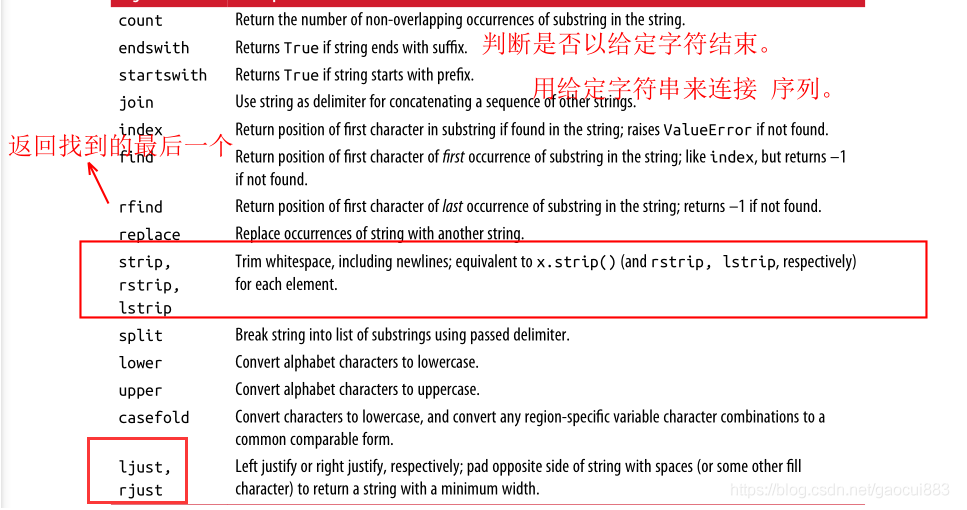
\includegraphics[width=\linewidth]{fig/na3}
	\caption{str相关操作}
	\label{fig-strcaozuo}
\end{figure}

\begin{figure}[htpb]
	\centering
	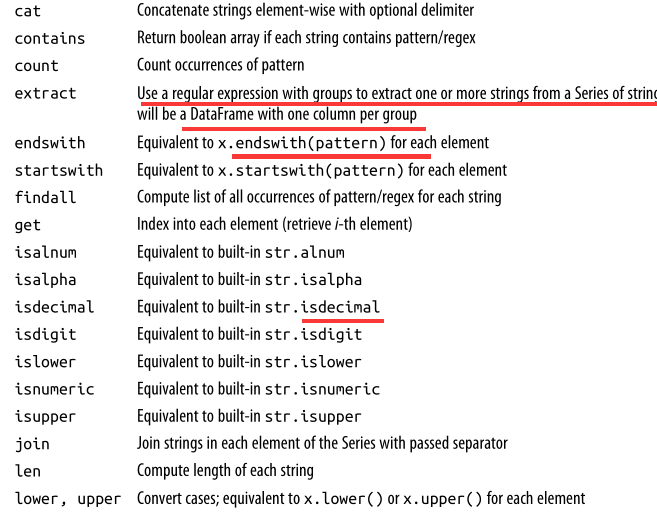
\includegraphics[width=\linewidth]{fig/a1}
	\caption{str和正则表达相关}
	\label{fig-reg}
\end{figure}


\section{数据的整理join,combine,reshpae}
\subsection{多重索引}
\begin{lstlisting}
	data = Series(np.random.randn(9), index = [['a', 'a', 'a', 'b', 'b', 'c', 'c', 'd', 'd'],
	[1, 2, 3, 1, 3, 1, 2, 2, 3]])
	
	data.unstack()
	data.unstack().stack()
	
	frame = DataFrame(np.arange(12).reshape((4, 3)),
	index=[['a', 'a', 'b', 'b'], [1, 2, 1, 2]],
	columns=[['Ohio', 'Ohio', 'Colorado'],
	['Green', 'Red', 'Green']])
	
	
	交换索引级别:
	swaplevel
	x.swaplevel('state','color',axis=1)
	frame.swaplevel('key1','key2',axis=0)
	排序:
	frame.sort_index(level=1,axis=0,ascending=True, inplace= False, kind='quicksort')
	
	frame.sort_index(level=0,axis=0,ascending=True, inplace= False, kind='quicksort')
	
	按索引级别分层统计:
	
	frame.sum(level='key2')
\end{lstlisting}

\subsection{setindex,resetincex}
\begin{lstlisting}
用列c做index索引:
	frame2 = frame.set_index(['c'])
多层索引:
    frame2 = frame.set_index(['c','d'])	
成为索引的同时丢弃原来:
	frame3 = frame.set_index(['c','d'], drop=False)	
默认将所有的index转换成index:
	frame4 = frame2.reset_index()
指定转换:	
	frame4 = frame2.reset_index(level=1, drop= False) 
\end{lstlisting}
\subsection{三大链接神奇:merge,jion,concat}
merge 是行方向,关键字相关链接,也就是根据索引或者列进行链接。
\begin{figure}[htpb]
	\centering
	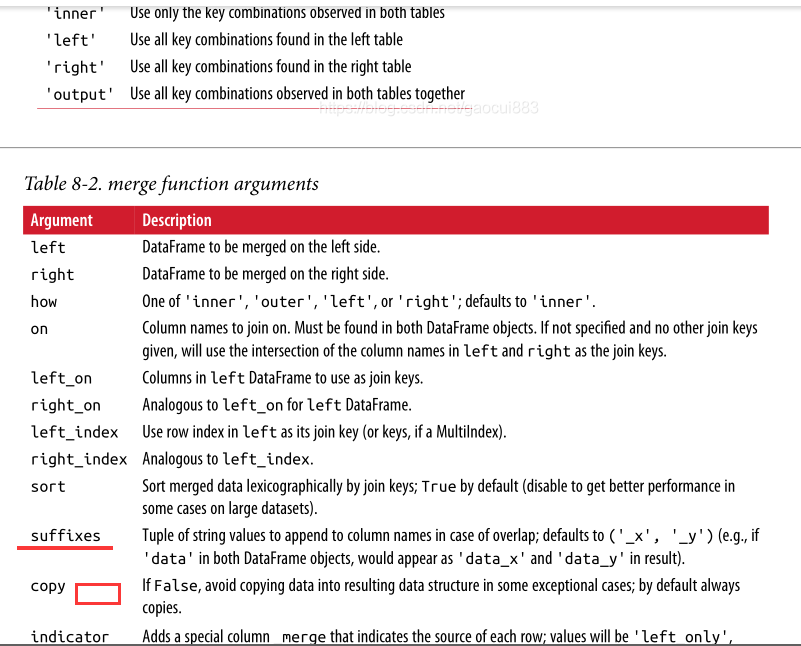
\includegraphics[width=\linewidth]{fig/a2}
	\caption{merge相关参数}
	\label{fig-merge}
\end{figure}
join 简单的将新的属性加入到原来的列表中即可。没有配对的设定为NAn\\
concat 列方向,竖直方向链接不同的表。\\

\begin{lstlisting}
	pd.merge(df1,df2)  # 默认对相同的名字的coloumn进行链接。
	# 也可对链接的名进行指定。
	pd.merge(df1,df2, on= 'key')
	
	df3 = pd.DataFrame({'lkey': ['b', 'b', 'a', 'c', 'a', 'a', 'b'],
	'data1': range(7)})
	
	df4 = pd.DataFrame({'rkey': ['a', 'b', 'd'],
	'data2': range(3)})
	
	pd.merge(df3,df4, left_on='lkey',right_on='rkey', how = 'inner')
	
	上边都是在一个列的基础上进行链接,也可以指定两个列:
	pd.merge(left,right, how='outer', on=['key1', 'key2'])
	
	如果非链接的多个列相同,那么可以设定后缀。
	pd.merge(left,right, how='outer', on=['key1'], suffixes=('_mother', '_dady'))
	
	按index和列名链接:
	pd.merge(left1,right1, left_on='key', right_on= None, left_index= False, right_index= True, how='outer')
	
	concat:
	
	pd.concat([s1,s2,s3], axis=1)
	链接后还可以设定高级索引:
	pd.concat([df1,df2], axis=1, keys=['level1', 'level2'])
	# 也可以传入字典,字典key 默认作为多层索引。
	pd.concat({'level1':df1, 'level2':df2}, axis=1)
	pd.concat([df1,df2], ignore_index=True, axis=0, keys=['df1','df2'])
	# 我们看到一个特别的情况, keys 不起作用了,这是因为 ignore_index.

	
\end{lstlisting}

\subsection{相同类型的表格的合并}


\begin{lstlisting}
	a = Series([np.nan, 2.5, np.nan, 3.5, 4.5, np.nan], index =['f', 'e', 'd', 'c', 'b', 'a'])
	
	b = Series(np.arange(len(a), dtype= np.float64), index=['f', 'e', 'd', 'c', 'b', 'a'])
	
	np.where(pd.isnull(a), b, a)  # pd.isnull 是条件,真选b,假选a
	等价于:
	b[:-2].combine_first(a[2:])
	dataframe类似:
	df1 = DataFrame({'a': [1., np.nan, 5., np.nan],
	'b': [np.nan, 2., np.nan, 6.],
	'c': range(2, 18, 4)})
	
	df2 = DataFrame({'a': [5., 4., np.nan, 3., 7.],
	'b': [np.nan, 3., 4., 6., 8.]})
	df1.combine_first(df2)
	
	
	
\end{lstlisting}

\subsection{reshpae,pivoting}
\begin{lstlisting}
	result = data.stack()
	行列进行交换:
	df.unstack('state').stack('side')
	透视表:
	pivoted = ldata.pivot('date', 'item', 'value')
	
\end{lstlisting}

\section{绘图和可视化}
	\subsection{初级教程}
	\begin{lstlisting}
		fig = plt.figure()
		ax1 = fig.add_subplot(2,2,1)
		ax2 = fig.add_subplot(2,2,2)
		ax3 = fig.add_subplot(2,2,3)
		
		plt.plot(np.random.randn(50).cumsum(), 'k--') #而这样的,则会默认在最后一个figure的最后一个subplot进行绘图。
		_ = ax1.hist(np.random.randn(100), bins=20, color='k', alpha=0.3) # alpha ??? 透明度。
		ax2.scatter(np.arange(30), np.arange(30)+3*np.random.randn(30))
		
		调整子图间距:
		subplots_adjust(left=None, bottom=None, right=None, top=None, wspace=None, hspace=None)
		
		
		fig,axes = plt.subplots(2,1)
		
		axes[0].plot(np.random.randn(20),np.random.randn(20),'g--')  # 绿色,虚线。折线。
		# more explictily as 
		axes[1].plot(np.random.randn(30),np.random.randn(30), linestyle='--', color='r')。
		
		from numpy.random import randn
		fig = plt.figure()
		ax = fig.add_subplot(1,1,1)
		ax.plot(randn(1000).cumsum(),'c',label='one')
		
		ax.plot(randn(1000).cumsum(), 'k--', label='two')
		ax.plot(randn(1000).cumsum(), 'r.', label='three')
		ax.legend(loc='best')
		
		
		
	\end{lstlisting}
	\begin{figure}[tbhp]
		\centering
		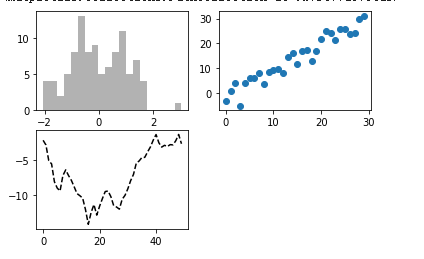
\includegraphics[width=\linewidth]{fig/p1}
		\caption{fig-plot1}
		\label{fig-shili}
	\end{figure}

\begin{figure}[tbhp]
	\centering
	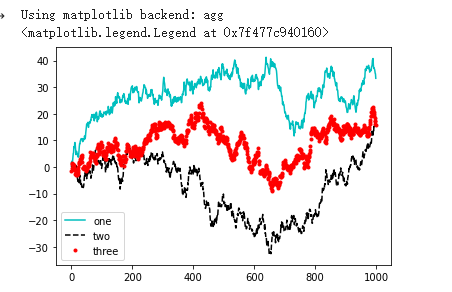
\includegraphics[width=\linewidth]{fig/p2}
	\caption{fig-plot2}
	\label{fig-shili2}
\end{figure}

\subsection[在图像上标记]{Annotations and Drawing on a Subplot}
\begin{lstlisting}
	fig = plt.figure()
	ax = fig.add_subplot(1,1,1)
	data = pd.read_csv('spx.csv', index_col=0, parse_dates = True)  # index_col 哪一列来做索引。parse_dates 
	spx = data['SPX']
	spx.plot(ax=ax, style='k-')
	
	crisis_data = [(datetime(2007, 10, 11), 'Peak of bull market'),
	(datetime(2008, 3, 12), 'Bear Stearns Fails'),
	(datetime(2008, 9, 15), 'Lehman Bankruptcy')]
	
	for date,label in crisis_data:
		ax.annotate(label, xy=(date, spx.asof(date)+75),  #spx.asof(date) ????
		xytext = (date,spx.asof(date)+225),
		arrowprops = dict(facecolor='black', headwidth=4, width=2,headlength=4),
		horizontalalignment='left',#水平对齐 
		verticalalignment='top') # 垂直对齐。
	ax.set_xlim(['1/1/2007','1/1/2011'])
	ax.set_ylim([600, 1800])
	ax.set_title('Important dates in the 2008-2009 financial crisis')
\end{lstlisting}

\begin{figure}[tbhp]
	\centering
	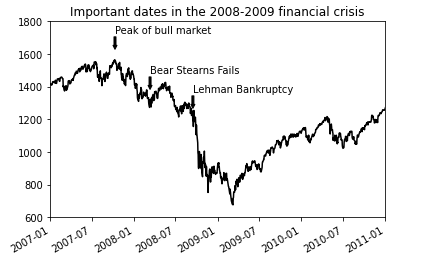
\includegraphics[width=\linewidth]{fig/p3}
	\caption{fig-plot3}
	\label{fig-shili3}
\end{figure}

\begin{lstlisting}
添加图形对象:
	rect = plt.Rectangle(xy = (0.2,0.75), width= 0.4, height= 0.5, alpha=0.3)
	circ = plt.Circle(xy=(0.7,0.2), radius=0.18, color='r', alpha=0.3)
	pgon = plt.Polygon(xy=[[0.15, 0.15], [0.35, 0.4], [0.2, 0.6]], color='c', alpha = 0.5)
	
	ax.add_patch(rect)
	ax.add_patch(circ)
	ax.add_patch(pgon)
	
\end{lstlisting}
\subsection{保存图片}
\begin{figure}[tbhp]
	\centering
	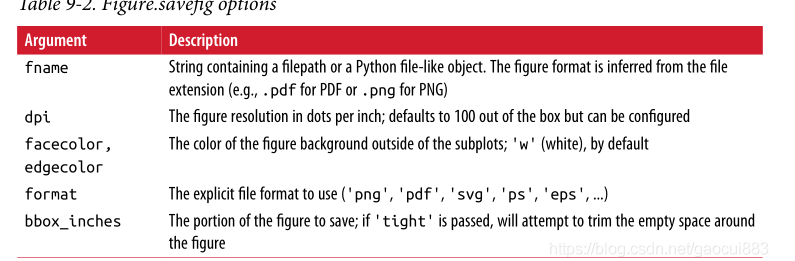
\includegraphics[width=\linewidth]{fig/p4}
	\caption{fig-plot4}
	\label{fig-shili4}
\end{figure}
\verb|plt.savefig(buffer)|

\subsection{用pandas和seaborn绘图}
series和pandas都可以直接用来绘图:
\begin{figure}[tbhp]
	\centering
	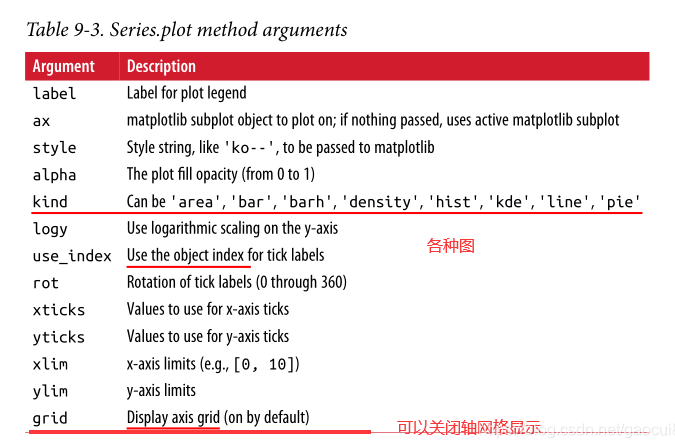
\includegraphics[width=\linewidth]{fig/p5}
	\caption{fig-plot5}
	\label{fig-shili5}
\end{figure}
\begin{figure}[tbhp]
	\centering
	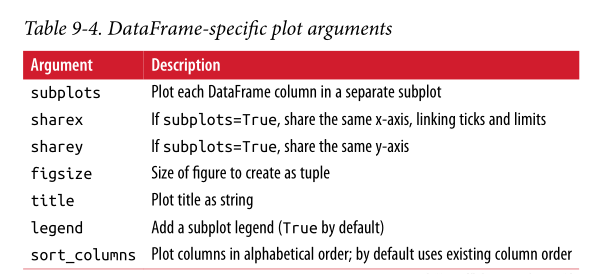
\includegraphics[width=\linewidth]{fig/p6}
	\caption{fig-plot6}
	\label{fig-shili6}
\end{figure}

\begin{lstlisting}
	# dataframe 默认会将每列化成线性图。
	
	# .plot() 还有很多其他options: use_index, xticks,xlim y_ticks,ylim.
	
	
	df = DataFrame(np.random.randn(10,4).cumsum(0), columns=['a','b','c','d'], index=np.arange(0,100,10))
	df.plot.bar()
	堆叠bar图:
	df.plot.bar(stacked = True)
	
seaborn:
	需要指定对应data,x,y
	sbn.barplot(x='tip_pct', y='day', data=tips, orient='h')
	
	
Histograms and Density Plots直方图和密度图:
	tips['tip_pct'].plot.hist(bins=30)
	tips['tip_pct'].plot.density()
	sbn.distplot(values, bins=100, color='r')
Scatter or Point Plots:
	 sbn.regplot('m1','unemp', data=trans_data)	
	 sbn.pairplot(trans_data, diag_kind='kde', plot_kws={'alpha':0.5})
\end{lstlisting}
\subsection{多维数据的绘图}
\begin{lstlisting}
	tips.head():
	total_bill	tip	smoker	day	time	size	tip_pct
	0	16.99	1.01	No	Sun	Dinner	2	0.063204
	1	10.34	1.66	No	Sun	Dinner	3	0.191244
	2	21.01	3.50	No	Sun	Dinner	3	0.199886
	3	23.68	3.31	No	Sun	Dinner	2	0.162494
	4	24.59	3.61	No	Sun	Dinner	4	0.172069
	
sbn.factorplot(x='day', y='tip_pct', hue='time', col='smoker', kind='bar', data=tips[tips.tip_pct < 1])

sbn.factorplot(x='day', y='tip_pct', row='time',
col='smoker',
kind='bar', data=tips[tips.tip_pct < 1])	

sbn.factorplot(x='tip_pct', y='day', kind='box',
data=tips[tips.tip_pct < 0.5])

sbn.factorplot ======sbn.catplot()
\end{lstlisting}


\begin{figure}[htpb]
	\centering
	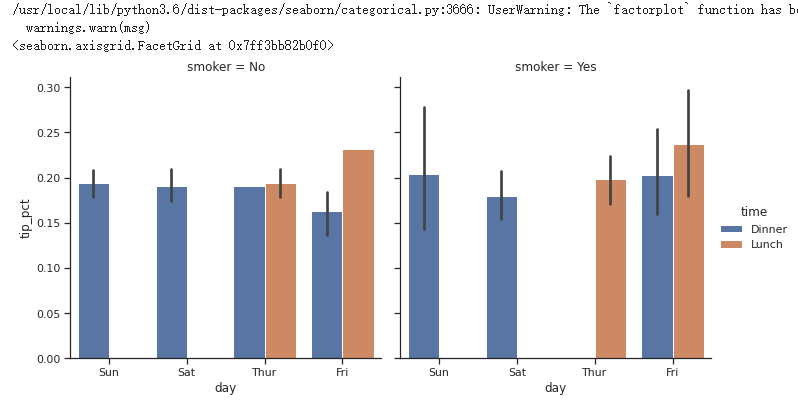
\includegraphics[width=\linewidth]{fig/p7}
	\caption{fig-plot7}
	\label{fig-shili7}
\end{figure}
\begin{figure}[htpb]
	\centering
	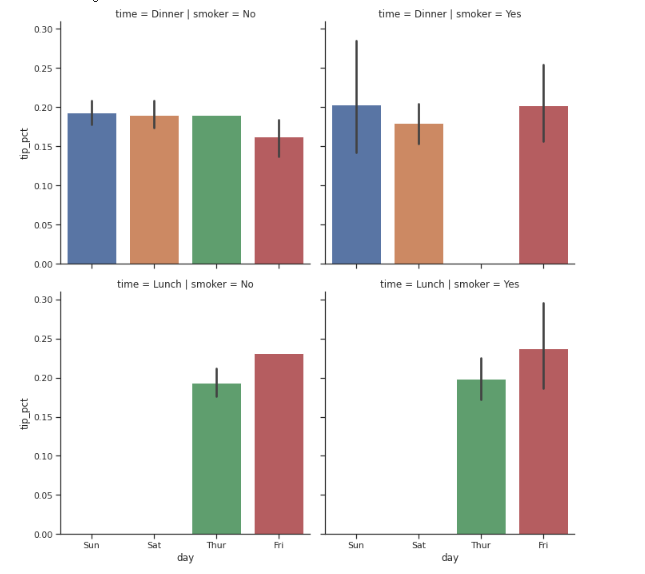
\includegraphics[width=\linewidth]{fig/p8}
	\caption{fig-plot8}
	\label{fig-shili8}
\end{figure}
\begin{figure}[htpb]
	\centering
	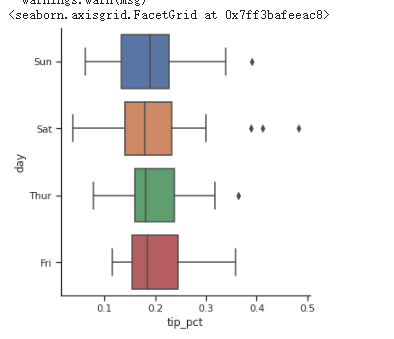
\includegraphics[width=\linewidth]{fig/p9}
	\caption{fig-plot9}
	\label{fig-shili9}
\end{figure}


\section[数据聚合分组操作]{Data Aggregation and Group Operations}
内容:对pandas 对象进行split,计算统计信息,应用groupby,\verb|pivot_table|,计算分位数分析信息。
\begin{figure}[htpb]
	\centering
	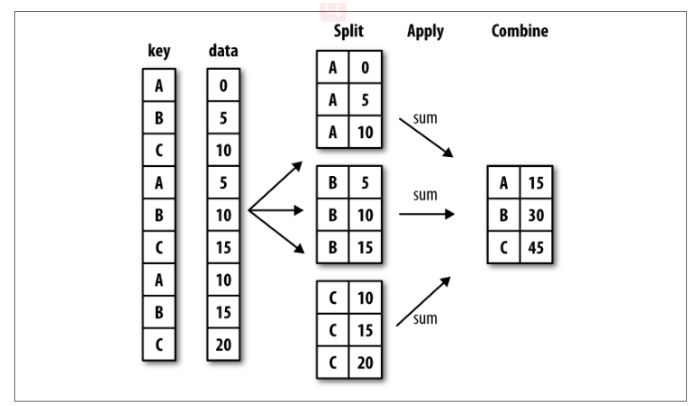
\includegraphics[width=\linewidth]{fig/p10}
	\caption{fig-plot10}
	\label{fig-shili10}
\end{figure}

\begin{lstlisting}
grouped = df['data1'].groupby(df['key1']) 
grouped
grouped.mean()
df['data1'].groupby([df['key1'],df['key2']]).mean()
key1  key2
a     one     0.296851
two     0.339220
b     one    -0.959031
two    -0.288006

df.groupby([df['key1'],df['key2']]).mean()
df.groupby(['key1','key2']).size()
可以迭代性:
for name, group in df.groupby(['key1']):
print(name)
print(group)


for (k1,k2), group in df.groupby(['key1','key2']):
print((k1,k2))
print(group)

pieces = dict(list(df.groupby('key1')))

注意以下两个的不同:
df.groupby('key1')['data1']
df.groupby('key1')[['data1']]

df.groupby(['key1','key2'])['data2'].mean()

mapping是一个字典:
by_column = people.groupby(mapping, axis=1)

series_column = people.groupby(map_series, axis=1).sum()

应用函数:
people.groupby(len).sum() #默认调用index,返回的数值用作新的index。
people.groupby([len, key_list]).min()

hier_df.groupby(level='cty', axis=1).mean()

def peaktopeak(arr):
return arr.max()-arr.min()

grouped.agg(peaktopeak)  # 注意agg或者aggregate
grouped.describe()
grouped = tips.groupby(['day', 'smoker'])
grouped_pct = grouped['tip_pct']
grouped_pct

grouped_pct.aggregate('mean')
grouped_pct.agg(['mean', 'std', peaktopeak])
# 如果我们要顺便改掉结果名呢???

# 传递一个元组的列表。
# 元组的第一个元素就是新的列名,第二个参数就是函数名。

grouped_pct.aggregate([('fuck1','mean'), ('fuck2','std'), ('fuck3', peaktopeak)])
# 如果是个DataFrame 呢。也就多个列。

functions =  ['count', 'mean', 'max']
result = grouped['tip_pct', 'total_bill'].agg(functions) # 对两列使用多个函数。
grouped.aggregate({'tip':[('fuck1','max'),('fuck2','min'),('fuck3','mean')], 'size':['sum','std']})

def top(df, n=5, column='tip_pct'):
	return df.sort_values(by=column)[-n:]  #找出最大的五个。
tips.groupby('smoker').apply(top) #  典型的split,apply, merge
tips.groupby('smoker').apply(top, n=3, column='tip')  # 这里的n和column都是top的参数。
a = tips.groupby(['smoker','day']).apply(top, n=1, column='tip')

\end{lstlisting}
\subsection{中位数和桶分析}
\begin{lstlisting}
	frame = DataFrame({'data1':np.random.randn(1000), 'data2':np.random.randn(1000)})
	quartiles = pd.cut(frame.data1, 4)
	quartiles.head()
	
# 然后计算每部分的最大,最小,均值,以及数据个数。

def get_stats(group):
	return {'min': group.min(),
	'max':group.max(),
	'mean':group.mean(),
	'count':group.count()}

grouped = frame.data2.groupby(quartiles)
x = grouped.apply(get_stats)
x.unstack()
根据group的数统计来填入缺失数据:
data.groupby(group_key).apply(lambda x: x.fillna(x.mean())) 


# 当然,如果提前准备好了相应的groupby对应的要填充的值也可以
fill_values = {'East':0.55555, 'West':-88888}

data.groupby(group_key).apply(lambda x : x.fillna(fill_values[x.name]))  #x.name


# Hearts, Spades, Clubs, Diamonds  #红桃,黑桃。梅花,方片。
suits = ['H', 'S', 'C', 'D']

card_val = (list(range(1, 11)) + [10] * 3) * 4

base_names = ['A'] + list(range(2, 11)) + ['J', 'K', 'Q']

cards = []

for suit in ['H', 'S', 'C', 'D']:

	cards.extend(str(num) + suit for num in base_names)  #对每个红桃对应每个数字。作为索引。

deck = pd.Series(card_val, index=cards)


def draw(deck, n=5):
	return deck.sample(n)
每个花色抽两张:
get_suit = lambda card: card[-1]
deck.groupby(get_suit).apply(draw, n=2)
	
	
	加权取均值:
	get_wavg = lambda x : np.average(x.data, weights= x.weights, axis= 0)
	
	grouped.apply(get_wavg)
	
	
	spx_corr = lambda x: x.corrwith(x['SPX']) # 其他列对spx列的贡献,或者相关度。
	rets = close_px.pct_change().dropna()
	get_year = lambda x: x.year 
	by_year = rets.groupby(get_year)#默认取索引,也就是年份。
	by_year.apply(spx_corr) #以年份来计算对指数收益的贡献。
\end{lstlisting}

\subsection{透视表}
\begin{lstlisting}
	tips.pivot_table?
	
	重要参数:
	values 要统计的透视的信息。
	index :纵向的指标。
	columns: 横向指标。
	aggfun: 统计透视函数。
	fill_value: 要替换na为什么值。
	
	# Signature: tips.pivot_table(values=None, index=None, columns=None, aggfunc='mean',
	# fill_value=None, margins=False, dropna=True, margins_name='All', observed=False) -> 'DataFrame'
	# Docstring:
	# Create a spreadsheet-style pivot table as a DataFrame.
	
	交叉表:
	交叉表是透视表的特例,计算频率。
	
	# pd.crosstab?
	# Signature: pd.crosstab(index, columns, values=None, rownames=None, colnames=None, aggfunc=None, margins=False, margins_name: str='All', dropna: bool=True, normalize=False) -> 'DataFrame'
	两个或者多个交叉信息。
	主要用来统计个数。
\end{lstlisting}

\section{时间序列}
时间索引类型:

时间戳。

时间段。

时间间隔。

累计时间间隔。

\begin{lstlisting}
	now = datetime.now()
	now.year
	delta = datetime(2011,1,5) - datetime(2010,2,3,12,8,3)
	from datetime import timedelta
	start = datetime(2011,1,7)
	
	x = start + timedelta(13)
	print(x)
	
	y = start - 2*timedelta(12)
	print(y)
	
	x.isocalendar() # 返回year,week,day.
	x.weekday() # 星期4.     0 - 6 星期1到天。
	x.ctime() # 返回一个日期字符串。
	x.strftime('%Y-%m-%d')
	
	
	stamp = datetime(2011, 1, 3)
	转化成特定格式的字符串:
	stamp.strftime('%Y-%m-%d')
	
	# 来识别特定格式的字符串时间序列。 
	# 关键字strptime  str pass time
	
	value = '2011-01-03'
	
	datetime.strptime(value, '%Y-%m-%d')
	
	datestrs = ['7/6/2011', '8/6/2011']
	
	[datetime.strptime(x, '%m-%d-%Y') for x in datestrs] 
	
	[datetime.strptime(x, '%m/%d/%Y') for x in datestrs]
	# 第三方库, dateutil 的时间解析库parser.parse 可以识别大部分人类能够识别的时间字符串格式。
	
	value = '2011-01-03'
	
	from dateutil.parser import parse
	
	value_date = parse(value)
	
	另一种,pandas自带的, pd.to_datetime()
	
	datestrs = ['2011-07-06', '2011-08-06']
	
	import pandas as pd
	
	pd.to_datetime(datestrs)
	
	时间段:
	pd.date_range(start=None, end=None, periods=None, freq=None, tz=None, normalize=False, name=None, closed=None, **kwargs) -> pandas.core.indexes.datetimes.DatetimeIndex
	
	ts.truncate(after='1/9/2011')  #截断,裁剪,丢弃的意思。
	Signature: ts.truncate(before=None, after=None, axis=None, copy: bool=True) -> ~FrameOrSeries
	
\end{lstlisting}
\begin{figure}[htpb]
	\centering
	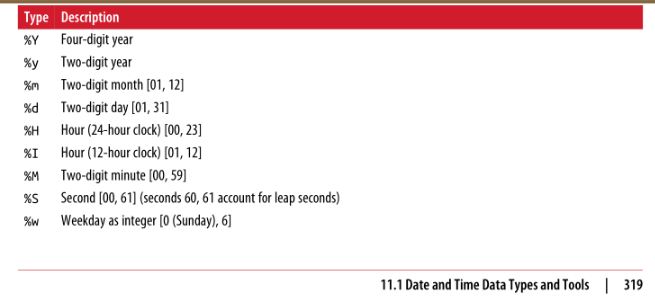
\includegraphics[width=\linewidth]{fig/t1}
	\caption{fig-t1}
	\label{fig-t1}
\end{figure}

\begin{figure}[htpb]
	\centering
	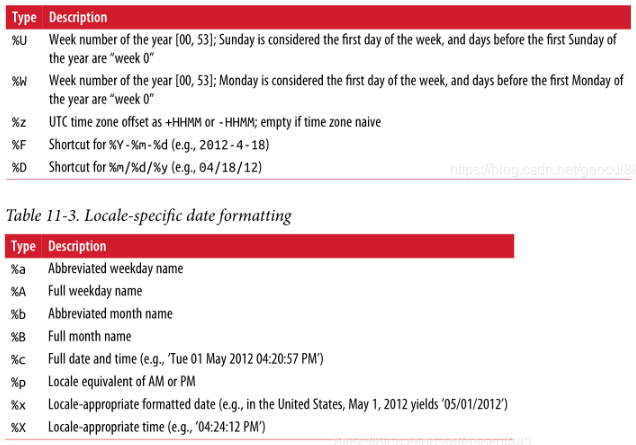
\includegraphics[width=\linewidth]{fig/t2}
	\caption{fig-plott2}
	\label{fig-shilit2}
\end{figure}


\subsection{Date Ranges, Frequencies, and Shifting}
\begin{lstlisting}
	index = pd.date_range('2012.04.01', '2012.06.01')
	from pandas.tseries.offsets import Hour, Minute
	
	fourhour = Hour(4)
	pd.date_range('2000.1.1', '2000.1.3', freq=fourhour)
	pd.date_range('2000.1.1', '2000.1.3', freq='4H')
	rng = pd.date_range('2012.1.1', '2012.9.1', freq='WOM-3FRI')# 每个月第三个星期五。
	
\end{lstlisting}
\begin{figure}[tbhp]
	\centering	
		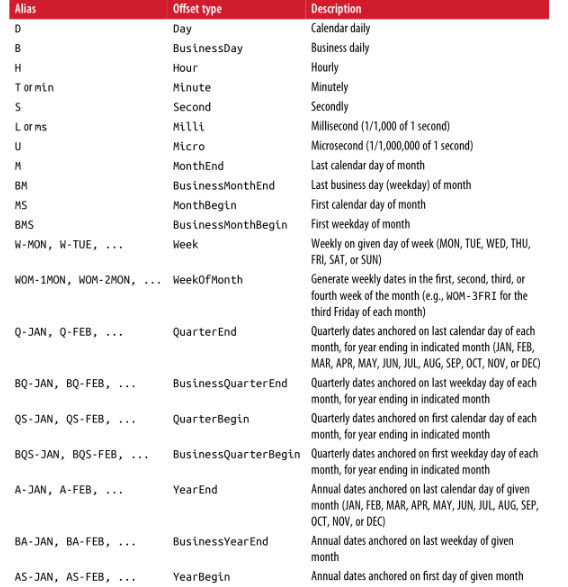
\includegraphics[width=\linewidth]{fig/t3}
		\caption{基础时间频率}
		\label{fig-timefreq}
\end{figure}


\subsection{shifting time}

\begin{lstlisting}
	ts = pd.Series(np.random.randn(4), index=pd.date_range('1/1/2000', periods=4, freq='M'))
	ts.shift(2)
	(ts-ts.shift(1))/ts.shift(1) # 可以很方便的计算两天的增长百分比。
	
	ts.shift(2,freq='M')
	ts.shift(2, freq='D')
	offset = MonthEnd()
	offset.rollforward(NOW) #显式的前滚。
	
	offset.rollback(NOW)
	
	ts = pd.Series(np.random.randn(20),
	index=pd.date_range('1/15/2000', periods=20, freq='4d'))
	
	ts.groupby(offset.rollforward).mean()
\end{lstlisting}
\subsection{时区设定}
\begin{lstlisting}
	import pytz
	pytz.common_timezones[-5:]
	tz = pytz.timezone('America/New_York')
	
	
	
	tz = pytz.timezone('America/New_York')
	rng = pd.date_range('3/9/2012 9:30', periods=6, freq='D')
	ts = pd.Series(np.random.randn(len(rng)), index=rng)
	ts_utc = ts.tz_localize('UTC')
	
	# 当然,也可以在生成的时候指定tz属性。
	pd.date_range('3/9/2011 9:30', periods=10, freq='D', tz='UTC')
	
	 将之前的是按转换为美国纽约时间。
	x = ts_utc.tz_convert('America/New_York')
	
	ts.index.tz_localize('Asia/Shanghai')
	
	stamp = pd.Timestamp('2011-03-12 04:00')
	stamp_utc = stamp.tz_localize('utc')
	stamp_utc.tz_convert('America/New_York')
	
	
\end{lstlisting}

\subsection{时间区间}

\begin{lstlisting}
	rng = pd.period_range('2001-01-01', '2002-05-01', freq='M')
	Signature: pd.period_range(start=None, end=None, periods=None, freq=None, name=None) -> pandas.core.indexes.period.PeriodIndex
	Docstring:
	Return a fixed frequency PeriodIndex.
	
	pd.period_range(start='2017-01-01', end='2018-01-01', freq='M')
	
	
	
	
\end{lstlisting}
\subsection{时间区间转换p.asfreq}
\begin{lstlisting}
	p.asfreq?
	Docstring:
	Convert Period to desired frequency, at the start or end of the interval.
	
	p.asfreq('M', how='start')
	p.asfreq('M', how='S') # s e 都是start和end的缩写。
	
	rng = pd.period_range('2006', '2009', freq='A-DEC')
	ts = pd.Series(np.random.randn(len(rng)), index=rng)
	
	ts.asfreq('M', how='S')
	

	
	
\end{lstlisting}

\subsection{季度周期}
\begin{lstlisting}
p = pd.Period('2012Q4', freq='Q-JAN')
p4pm = (p.asfreq('B', 'e') -1).asfreq('T','s') + 16*60 # 表示分钟。s表示start 
rng = pd.period_range('2011Q3','2012Q4', freq='Q-JAN')
PeriodIndex(['2011Q3', '2011Q4', '2012Q1', '2012Q2', '2012Q3', '2012Q4'], dtype='period[Q-JAN]', freq='Q-JAN')

ts = pd.Series(np.arange(len(rng)), index=rng)
new_rng = (rng.asfreq('B','e') -1).asfreq('T','s')+16*60
ts.index = new_rng.to_timestamp()


pts = ts.to_period()
ts2.to_period('M').to_timestamp(how='start') #可以转回去。
将不同列的时间信息组合起来:
index = pd.PeriodIndex(year=data.year, quarter=data.quarter, freq='Q-DEC')



\end{lstlisting}
\subsection{时间采样,上下混合采样等}
\begin{lstlisting}
	rng = pd.date_range('2000-01-01', periods=100, freq='D')
	ts = pd.Series(np.random.randn(len(rng)), index=rng)
	ts.resample?
	Signature: ts.resample(rule, axis=0, closed: Union[str, NoneType]=None, label: Union[str, NoneType]=None, 
	convention: str='start', kind: Union[str, NoneType]=None, 
	loffset=None, base: int=0, on=None, level=None)
	
	一般采样后都进行统计 resample().sum()/fill()/apply()/asfreq()/
	# 计算一个bins内的first(open), last(close), maximum(high)
	
	 minimal(low)四个数据。
	# 公式:ohlc 
	
	ts.resample('M').ohlc()
	annual_frame.resample('Q-DEC').ffill() 
	annual_frame.resample('Q-DEC', convention='end').ffill()
	
	
	
\end{lstlisting}

\subsection{滑动窗口rolling()}
\begin{lstlisting}
	close_px_all = pd.read_csv('stock_px_2.csv', parse_dates=True, index_col=0)
	close_px = close_px_all[['AAPL', 'MSFT', 'XOM']]
	close_px = close_px.resample('B').ffill()
	
	
	close_px.AAPL.plot()
	close_px.AAPL.rolling(250).mean().plot() # 滑动窗口的平均。类似于groupby 和 resample ,调用后可以调用统计函数。
	
	# 一个问题,在开始阶段,我们数据可能少于window periods 怎么设置???
	# min_periods 这个参数可以
	
	appl_std250 = close_px.AAPL.rolling(250, min_periods=10).std()
	
	close_px.AAPL.rolling(window, min_periods=None, center=False, win_type=None, on=None, axis=0, closed=None)
	
	
	# expanding 从窗口从小到大,知道最后充满整个序列。
	
	expending_mean = appl_std250.expanding().mean()
	
close_px:
	AAPL	MSFT	XOM
	2003-01-02	7.40	21.11	29.22
	2003-01-03	7.45	21.14	29.24
	2003-01-06	7.45	21.52	29.96
	2003-01-07	7.43	21.93	28.95
	2003-01-08	7.28	21.31	28.83
	...	...	...	...
	2011-10-10	388.81	26.94	76.28
	2011-10-11	400.29	27.00	76.27
	2011-10-12	402.19	26.96	77.16
	2011-10-13	408.43	27.18	76.37
	2011-10-14	422.00	27.27	78.11
close_px.rolling(60).mean().plot(logy=True)
	
	
\end{lstlisting}

\begin{figure}[tbhp]
	\centering
	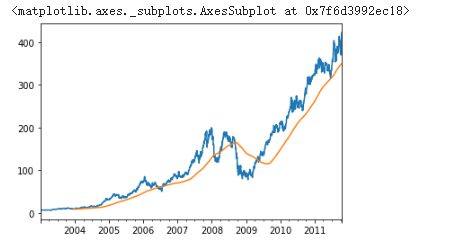
\includegraphics[width=\linewidth]{fig/t4}
	\caption{时间滑动窗口}
	\label{fig-timeswap}
\end{figure}

\begin{figure}[tbhp]
	\centering
	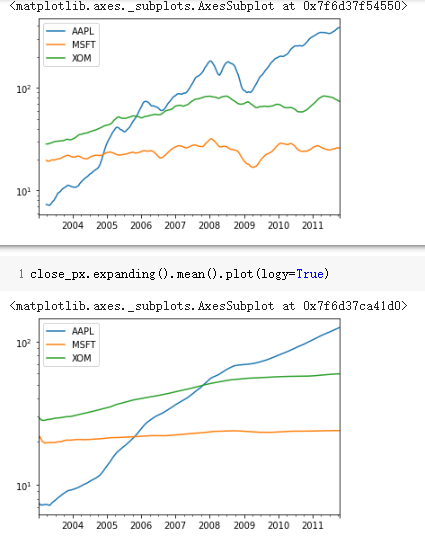
\includegraphics[width=\linewidth]{fig/t5}
	\caption{画图对象是DATAFRAME对象的时候}
	\label{fig-rollingdataframe}
\end{figure}

\subsection{指数加权函数}

\begin{lstlisting}
	appl_px = close_px.AAPL['2006':'2007']
	
	ma60 = appl_px.rolling(30, min_periods=20).mean()
	
	ma60x = appl_px.rolling(30, min_periods=20)
	
	max60gaussian = appl_px.rolling(30, min_period=20, win_tpye='guassian').mean(std = 3)
	
	ewma60 = appl_px.ewm(span=30).mean() #指数加权。
	
	
	
	# 我们之前都是用的mean,sum函数,其实也可以自定义函数,要注意的就是,函数是从一个list返回一个标量即可。
	
	from scipy.stats import percentileofscore
	score_at_2percent = lambda x: percentileofscore(x, 0.02)
	reslult = returns.AAPL.rolling(250).apply(score_at_2percent)
	reslult.plot()
	
\end{lstlisting}

\section{pandas 高级部分}

\subsection{分类类类型categorical}
更好的性能和内存使用,在分类数据或者机器学习的应用中

\begin{lstlisting}
	# 关键词: 
	# Categorical
	# astype('category') 将类型转换为pandas.Categorical 对象。
	# 
	# 属性: values.categories && values.codes
	# # 直接建立Categorical 对象。 pandas.Categorical() 类似于 dataframe,series.
	
	# # 也可以指定 相应的代码。
	# categories = [xxx]
	# codes = [xx]
	# my_cats_2 = pd.Categorical.from_codes(codes, categories, ordered = Ture or False)
	
	
	fruit_cat = df.fruit.astype('category')
	
	# frome codes 建立。
	categories = ['foo', 'bar', 'baz']
	codes = [0,1,2,0,0,1]
	
	my_cat = pd.Categorical.from_codes(codes, categories, ordered=True)
	my_cat
	
	
\end{lstlisting}


\subsection{categorical 类型的计算效率}


\begin{lstlisting}
	pd.qcut 产生的 categorical对象。
	# 可以直接用 .codes && categories 属性访问。
	# 可以设置label 来修改输出的结果。
	# bins = pd.qcut(list, 4, label=['x1','x2','x3','x4'])
	# 然后对bins 进行 groupby,统计相应的值。因为groupby可以直接传入一个维度或者长度于对应列数相同的列表或者series.
	# 性能提升: 当用字符串存储的时候,和用 categorical 对象存储的时候,所占用的内存大小完全不一样。
	# 当然,在这个基础上用groupby等运算的时候,所用的时间也不一样。
	
	
	draws = np.random.randn(1000)
	# 上边的1000个数,进行qcut,根据大小范围,四份。
	bins = pd.qcut(draws, 4)
	
	# 从结果看出,bins拥有categories的属性。
	# 我们来用categories && codes来访问
	
	bins.categories
	
	
	用bins来对draws进行groupby并进行一些统计输出
	bins = pd.Series(bins, name='quartile')
	
	resluts = pd.Series(draws).groupby(bins).agg(['count', 'min', 'max', 'mean']).reset_index()
	
	# 然后我们可以查看,categorical 对象和 字符对象占用内存对比。
	
	N = 10000000
	draws = pd.Series(np.random.randn(N))
	labels = pd.Series(['foo', 'bar', 'baz', 'qux'] * (N // 4))
	
	# 将series 转换成categorical 
	
	categories = labels.astype('category')
	
	labels.memory_usage()/categories.memory_usage()
	7.999756807782151
	%time _=labels.astype('category')
	CPU times: user 377 ms, sys: 4.52 ms, total: 382 ms
	Wall time: 383 ms
	
	
	# cat 提供了对访问codes categories 的方法。
	
	# cat.set_categories() 来扩展类别对象,虽然只是观察到了有限个。
	# 比如没有观察到的类比依然会统计信息统计到,只是个数为0而已。 value_counts...
	
	# 大型数据集中,很多类别没有使用,想要去掉这些没有观察到的类别,使用: remove_unused_categories.
	
	
	# 哑变量: 转换: pandas.get_dummies(series)
	cat_s2.cat.remove_unused_categories()
	cat_s2 = cat_s.cat.add_categories(['e'])
	pd.get_dummies(cat_s) 
	
	
	
\end{lstlisting}

	\section{groupby 更加高级的用法}
	
\begin{lstlisting}
	df = pd.DataFrame({'key': ['a', 'b', 'c'] * 4,
	'value': np.arange(12.)})
	
	g = df.groupby('key').value
	
	g.transform(lambda x: x.mean())
	g.transform('mean')
	g.apply(lambda x:x*2)====
	g.transform(lambda x:x.rank(ascending=False))
	
	normalized = (df['value'] - g.transform('mean'))/g.transform('std')
	
	时间序列数据,resample类似于groupby,但是当dataframe的时候,需要使用TimeGrouper
	
	# 想要对df2 的key和time都进行groupby操作,该如何进行?
	df2.groupby('key').resample('5min', on='time').sum()
			value
	key	time	
	a	2017-05-20 00:00:00	30.0
	2017-05-20 00:05:00	105.0
	2017-05-20 00:10:00	180.0
	b	2017-05-20 00:00:00	35.0
	2017-05-20 00:05:00	110.0
	2017-05-20 00:10:00	185.0
	c	2017-05-20 00:00:00	40.0
	2017-05-20 00:05:00	115.0
	2017-05-20 00:10:00	190.0
	
	
	
	df2.groupby('key').resample('5min', on='time').sum().reset_index()
	
\end{lstlisting}
\end{document}

